%%%%%%%%%%%%%%%%%%%%%%%%%%%%%%%%%%%%%%%%

% PDF compatibility code. 



\makeatletter
\newif\ifpdflatex@
\ifx\pdftexversion\@undefined
\pdflatex@false
%\message{Not using pdf}
\else
\pdflatex@true
%\message{Using pdf}
\fi

\newcommand{\latexpdf}[2]{
  \ifpdflatex@ #1
  \else #2
  \fi
}

\newcommand{\latexorpdf}[2]{
  \ifpdflatex@ #2
  \else #1
  \fi
}

\newcommand{\pformat}{a4paper}

\makeatother

%%%%%%%%%%%%%%%%%%%%%%%%%%%%%%%%%%%%%%%%

\latexorpdf{
\documentclass[\pformat,12pt]{jarticle}
}{
% pdftex option is used by graphic[sx],hyperref,toolbox.sty
\documentclass[\pformat,pdftex,12pt]{jarticle}
}

\usepackage{toolbox}
\usepackage{makeidx}
\usepackage{here}
\usepackage{verbatimfiles}
\usepackage{ifthen}
\usepackage{longtable}
\usepackage{array}

% Ueki change start
\ifnum 42146=\euc"A4A2 \AtBeginDvi{\special{pdf:tounicode EUC-UCS2}}\else
\AtBeginDvi{\special{pdf:tounicode 90ms-RKSJ-UCS2}}\fi

\usepackage[dvipdfm,bookmarks=true,bookmarksnumbered=true,colorlinks,plainpages=true]{hyperref}
\usepackage{cite}

\def\seename{$\Rightarrow$}
% Ueki change end

% Ueki delete start
%\latexorpdf{
%\usepackage[plainpages=true,colorlinks,linkcolor=black,citecolor=black,pagecolor=black, urlcolor=black]{hyperref}
%}{
%\usepackage[plainpages=true,colorlinks]{hyperref}
%}
% Ueki delete end

\usepackage{color}
\newcommand{\vdmsl}{VDM-SL }
\newcommand{\vdmpp}{VDM++ }

\makeindex


% Following command used to preserve backslash in tabular environments
\newcommand{\pbs}[1]{\let\temp=\\#1\let\\=\temp}

\newenvironment{interfacetable}{%
  \begin{longtable}{|>{\pbs\raggedright\ttfamily}p{6.6cm}%
                    |>{\pbs\raggedright}p{6.6cm}|} \hline
  \textrm{\bfseries 名称} &  \textbf{説明} \\ \hline
  \endhead
  }{\end{longtable}}

\newcommand{\APIError}{\hyperlink{exception.APIError}{raises APIError}}
\newcommand{\VDMError}{\hyperlink{exception.VDMError}{raises VDMError}}
\newcommand{\Generic}{\hyperlink{interface.Generic}{Generic}}
\newcommand{\VDMGeneric}{\hyperlink{interface.Generic}{VDMGeneric}}
\newcommand{\ModuleName}{\hyperlink{type.ModuleName}{ModuleName}}
\newcommand{\ModuleList}{\hyperlink{type.ModuleList}{ModuleList}}
\newcommand{\ClassName}{\hyperlink{type.ClassName}{ClassName}}
\newcommand{\ClassList}{\hyperlink{type.ClassList}{ClassList}}
\newcommand{\FileName}{\hyperlink{type.FileName}{FileName}}
\newcommand{\FileList}{\hyperlink{type.FileList}{FileList}}
\newcommand{\ToolType}{\hyperlink{type.ToolType}{ToolType}}
\newcommand{\ErrorStruct}{\hyperlink{struct.Error}{Error}}
\newcommand{\ModuleStatus}{\hyperlink{struct.ModuleStatus}{ModuleStatus}}
\newcommand{\VDMApplication}{\hyperlink{interface.VDMApplication}{VDMApplication}}
\newcommand{\VDMCodeGenerator}{\hyperlink{interface.VDMCodeGenerator}{VDMCodeGenerator}}
\newcommand{\VDMErrors}{\hyperlink{interface.VDMErrors}{VDMErrors}}
\newcommand{\VDMInterpreter}{\hyperlink{interface.VDMInterpreter}{VDMInterpreter}}
\newcommand{\VDMModuleRepos}{\hyperlink{interface.VDMModuleRepos}{VDMModuleRepos}}
\newcommand{\VDMFactory}{\hyperlink{interface.VDMFactory}{VDMFactory}}
\newcommand{\VDMParser}{\hyperlink{interface.VDMParser}{VDMParser}}
\newcommand{\VDMPrettyPrinter}{\hyperlink{interface.VDMPrettyPrinter}{VDMPrettyPrinter}}
\newcommand{\VDMProject}{\hyperlink{interface.VDMProject}{VDMProject}}
\newcommand{\VDMTypeChecker}{\hyperlink{interface.VDMTypeChecker}{VDMTypeChecker}}
\newcommand{\ClientID}{\hyperlink{type.ClientID}{ClientID}}
\newcommand{\bytes}{\hyperlink{type.bytes}{bytes}}
\newcommand{\VDMBool}{\hyperlink{interface.VDMBool}{VDMBool}}
\newcommand{\VDMChar}{\hyperlink{interface.VDMChar}{VDMChar}}
\newcommand{\VDMNumeric}{\hyperlink{interface.VDMNumeric}{VDMNumeric}}
\newcommand{\VDMQuote}{\hyperlink{interface.VDMQuote}{VDMQuote}}
\newcommand{\VDMText}{\hyperlink{interface.VDMText}{VDMText}}
\newcommand{\VDMToken}{\hyperlink{interface.VDMToken}{VDMToken}}
\newcommand{\VDMNil}{\hyperlink{interface.VDMNil}{VDMNil}}
\newcommand{\VDMMap}{\hyperlink{interface.VDMMap}{VDMMap}}
\newcommand{\Map}{\hyperlink{interface.VDMMap}{Map}}
\newcommand{\VDMRecord}{\hyperlink{interface.VDMRecord}{VDMRecord}}
\newcommand{\Record}{\hyperlink{interface.VDMRecord}{Record}}
\newcommand{\VDMSequence}{\hyperlink{interface.VDMSequence}{VDMSequence}}
\newcommand{\Sequence}{\hyperlink{interface.VDMSequence}{Sequence}}
\newcommand{\VDMSet}{\hyperlink{interface.VDMSet}{VDMSet}}
\newcommand{\Set}{\hyperlink{interface.VDMSet}{Set}}
\newcommand{\VDMTuple}{\hyperlink{interface.VDMTuple}{VDMTuple}}
\newcommand{\Tuple}{\hyperlink{interface.VDMTuple}{Tuple}}
  
% Following command used to put notes in drafts to remind author of
% incomplete parts
\newcommand{\note}[1]{\colorbox{red}{#1}}

\makeatletter
% ------------- TOC manipulation ------------
\def\docglbldepth{1}
%\setcounter{secnumdepth}{\docglbldepth}
%\setcounter{tocdepth}{\docglbldepth}
\def\@pnumwidth{3.0em}
% more space for for >10 subsections
%\def\l@section{\@dottedtocline{1}{1.5em}{3.1em}}
\def\l@subsection{\@dottedtocline{2}{1.5em}{2.8em}}
%\def\l@subsubsection{\@dottedtocline{3}{4.3em}{3.6em}}
%\def\l@paragraph{\@dottedtocline{4}{7.9em}{4.1em}}
%\def\l@subparagraph{\@dottedtocline{5}{10em}{5em}}
\makeatother

\makeindex


\begin{document}

\vdmtoolsmanualscsk{VDMTools APIマニュアル}{2.0}

\renewcommand{\thepage}{\roman{page}}

%\tableofcontents
\label{endtofc}
\ifthenelse{\isodd{\pageref{endtofc}}}{\mbox{}\newpage}{}
\newpage 
\renewcommand{\thepage}{\arabic{page}}
\setcounter{page}{1}


\section{導入}
本書は、VDM Toolboxに含まれるCORBA対応APIの使い方について記述したものである。

VDM Toolbox API では、グラフィカルな画面からあるいはコマンドラインから、VDM Toolbox 実行インスタンスの一定プロパティの参照や修正を行うような、クライアントプログラムの作成が許されている。
 VDM Toolbox では、同時に複数の CORBA クライアントからのアクセスが可能である。
これらクライアントは API を通して、プロジェクトにアクセスし設定を行う、個々のファイルの構文分析や型検査をする、インタープリタを通した式評価を行う、等々が可能である。
クライアントプロセスと VDM Toolboxは分離したプロセスであり、ネットワーク上の異なるマシン上において、場合によっては異なるオペレーティングシステム上で、実行され得るものである。
その結果、 あるクライアントプロセスでサーバーとして用いられているVDM Toolboxを、ユーザーインターフェースを通してこのユーザーが利用できる。

 API は CORBA (see \cite{OMG&96})を基本とする。
この理由により、 CORBA2.0準拠実装を行う言語ならばこのAPIへのアクセスが可能である。
たとえば C++ か Javaで簡単にクライアントの記述が可能であるが、それはこれらの言語に対しては、フリーのものを含めいくつかのCORBAが実装可能だからである。
第~\ref{Toolboxapi}章では、C++で書かれた小さな例題コードが提供される。
しかし第~\ref{writingacppclient}章と \ref{writingajavaclient}章では、C++ と Java各々で完全なクライアントの記述法を述べる。

本書と本書で述べるAPIは、 ToolboxのVDM-SL版とVDM++版の双方へ適用される。 
ほんのわずかなケースにおける、 APIのVDM-SLとVDM++間での相違については、はっきりとAPIの定義に述べられている。
このマニュアル中での``module"は一般的に、VDM-SLにおけるモジュールまたはVDM++におけるクラスを示している。

\newpage
\section{CORBA - 基本原則}

CORBA の本旨は {\em オブジェクトの分散}である。
クライアントプロセスは、ネットワーク上にローカルあるいはリモートに配置された別々のサーバープロセスで取り扱われ物理的に保存されたオブジェクトに対して、状態を再現し、それにアクセスし、場合によっては修正したりすることができる。
クライアントはサーバー中に保存されたオブジェクトに対して ``ハンドル'' を持ち、あたかも分散オブジェクトがクライアントのアドレス空間に配置されているかのように、 このハンドルをメソッドの呼び出しに用いる。
 CORBA 標準仕様では、メソッドの発動方法や異なるオブジェクト間での値のやり取りの方法と同様に、どのように分散オブジェクトに対するハンドルを獲得できるかについての仕様を定めている。

 CORBA は単にオブジェクト分散に対する標準であるため、CORBA サーバーおよびクライアントを記述するためにはCORBA の実装(いわゆる {\em ORB}) が必要である。
現在においてCORBA 実装は、異なるプラットフォームや言語の多くに対して利用可能である。  

\subsection{IDL}

サーバーで動作しCORBA で公開されるオブジェクトは、インターフェイス定義言語(IDL)を用いて記述される。
IDL は、実装向き言語でプラットフォームに中立にインターフェイスを記述するための、オブジェクト指向言語である。
CORBAインターフェイスを持つツールを提供するベンダーは、顧客にそのツールと共にIDL記述を配布することでこのインターフェイスの存在を知らせている。
IDL の文法は \cite{OMG&96}に記述されている。 

クライアント実装を行うとき、IDL記述はIDLコンパイラ(選択されたCORBA実装に伴って提供される)により、任意に選択された実装言語にマップされる。
 IDL記述から生成されるコードはコンパイルされ、サーバーのCORBAインターフェイスを用いることができた実行可能なクライアントと共にリンクされる。

\newpage
\section{VDM Toolbox API(アプリケーションインターフェイス)} 
\label{Toolboxapi}

VDM Toolbox のCORBAインターフェイスは、2つの IDLファイル {\tt corba\_api.idl} と {\tt metaiv\_idl.idl}で記述されていて、VDM Toolboxと共に分散配布される。
1番目のファイルでは実際のVDM Toolboxのインターフェイスが記述され、2番目のファイルではクライアントとVDM Toolbox間でやり取りされるさまざまなVDM値のインターフェイスが記述されている。
以下で両ファイルの詳細を述べ、第~\ref{refguide}章でこれらインターフェイスの参照マニュアルを提供する。

\subsection{APIツールのIDL記述}
\label{idldescriptiontool}

VDM ToolboxのAPIは、クライアントプロセスからアクセス可能な多くの様々なオブジェクト(IDLにおけるインターフェイス)から構成される。
オブジェクトである {\tt  \VDMApplication}メインの入口であり、ここからAPIの他のインターフェイスすべての利用が可能である。
このオブジェクトは VDM Toolboxへのクライアントハンドルであり、APIの他の任意の機能の利用に先立ち構築されている必要がある。
第~\ref{writingacppclient} 章と第~\ref{writingajavaclient}章で、C++と Java各々においてVDM Toolboxに対するこのハンドルをどう獲得するかを述べる。

%\begin{figure}[tbh]
%\begin{center}
%\mbox{}
%\resizebox{6cm}{!}{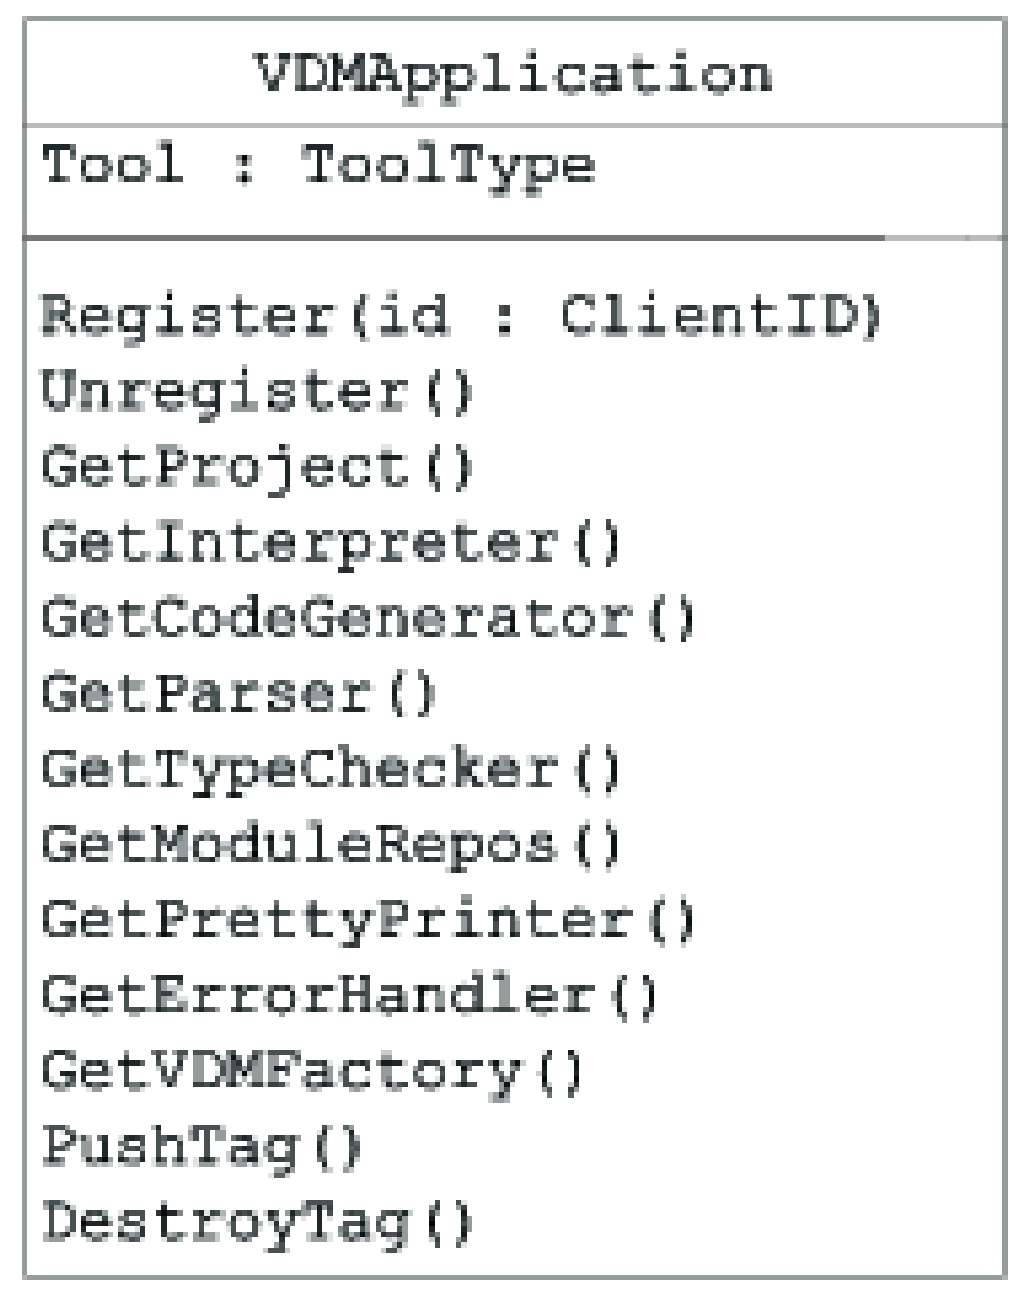
\includegraphics{VDMApplication}}
%\caption{The {\tt VDMApplication} interface.}\label{fig:VDMApplication}
%\end{center}
%\end{figure}

\begin{figure}[tbh]
\begin{center}
\begin{tabular}{|l|}
\hline
{\tt ToolboxAPI::VDMApplication } \\
\hline
{\tt Tool: ToolType } \\
\hline
{\tt Register () } \\
{\tt Unregister(in VDM::ClientID id) } \\
{\tt GetProject() }\\
{\tt GetInterpreter() }\\
{\tt GetCodeGenerator() }\\
{\tt GetParser() }\\
{\tt GetTypeChecker() }\\
{\tt  GetPrettyPrinter() }\\
{\tt GetErrorHandler() }\\
{\tt GetModuleRepos() }\\
{\tt GetVDMFactory() }\\
{\tt PushTag(in VDM::ClientID id) }\\
{\tt DestroyTag(in VDM::ClientID id) }\\
\hline
\end{tabular}
\caption{{\tt VDMApplication} インターフェイス}\label{fig:VDMApplication}
\end{center}
\end{figure}

 {\tt \VDMApplication} インターフェイスを図~\ref{fig:VDMApplication}に示す。  
メソッド {\tt Register} と {\tt  Unregister} は、サーバー上での処理を登録および解除するために、クライアントによって用いられる。
 {\tt \VDMApplication} インターフェイスはさらにたくさんの、他のインターフェイスをリターン値として戻すメソッドから構成されている。
たとえばVDM Toolboxで最新プロジェクトを構成しようと望むなら、そのプロジェクトインターフェイスに対するハンドル、これは以下で述べる {\tt \VDMProject}インターフェイスのハンドルである、を得るため {\tt GetProject} を用いるべきである。
加えて、インターフェイスの{\tt Tool} 属性は、サーバーとして用いるツール型、つまりクライアントが VDM-SL と VDM++ Toolboxのどちらに接続されているか、を決定するのに用いることができる。

\subsubsection{VDMProject}

%\begin{figure}[tbh]
%\begin{center}
%\mbox{}
%\resizebox{7.5cm}{!}{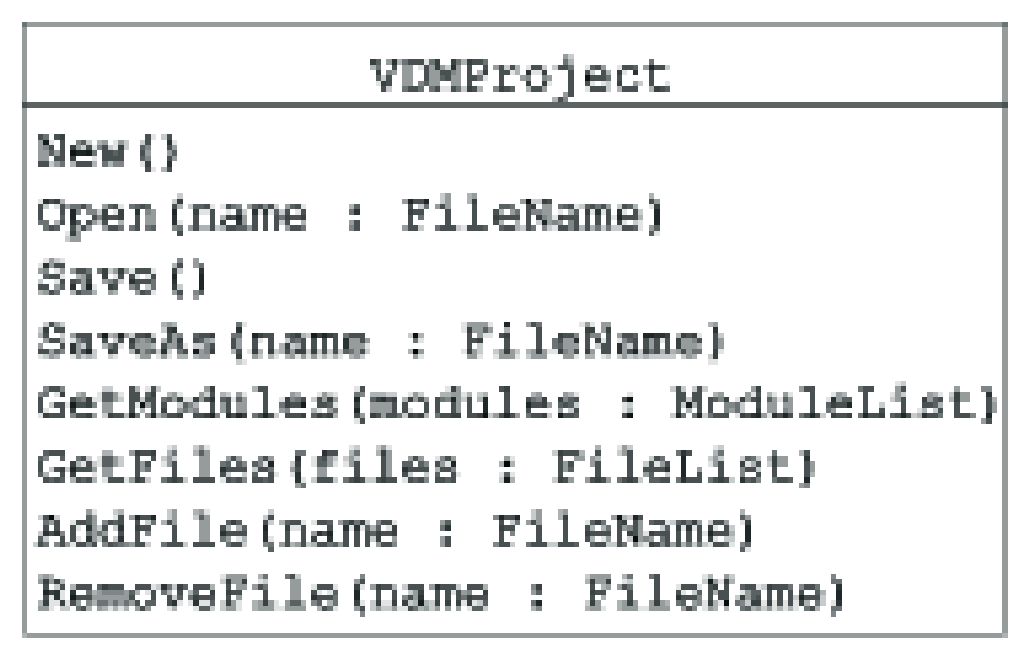
\includegraphics{VDMProject}}
%\caption{The {\tt VDMProject} interface.}\label{fig:VDMProject}
%\end{center}
%\end{figure}

\begin{figure}[tbh]
\begin{center}
\begin{tabular}{|l|}
\hline
{\tt ToolboxAPI::VDMProject } \\
\hline
{\tt New() } \\
{\tt Open(in FileName name) } \\
{\tt Save() } \\
{\tt SaveAs(in FileName name) } \\
{\tt GetModules(out ModuleList modules)} \\
{\tt GetFiles(out FileList files)} \\
{\tt AddFile(in FileName name)} \\
{\tt RemoveFile(in FileName name)} \\
\hline
\end{tabular}
\caption{{\tt VDMProject} インターフェイス}\label{fig:VDMProject}
\end{center}
\end{figure}

 {\tt \VDMProject}インターフェイスを図~\ref{fig:VDMProject}に示す。
このインターフェイスを用いて、VDM Toolboxの最新プロジェクトへのアクセスと修正が可能となる。 
{\tt GetFiles} と {\tt GetModules}は、最新プロジェクトのファイル名とモジュール名の列を(パラメーターを通して) 返す。
{\tt  AddFile} と {\tt RemoveFile} はプロジェクト構成に用いられる。

\subsubsection{VDMModuleRepos}

{\tt \VDMModuleRepos} インターフェイスを図~\ref{fig:VDMModuleRepos}に示す。

%\begin{figure}[tbh]
%\begin{center}
%\mbox{}
%\resizebox{15cm}{!}{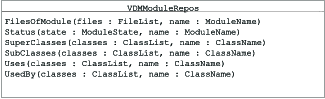
\includegraphics{VDMModuleRepos}}
%\caption{The {\tt VDMModuleRepos} interface.}\label{fig:VDMModuleRepos}
%\end{center}
%\end{figure}

\begin{figure}[tbh]
\begin{center}
\begin{tabular}{|l|}
\hline
{\tt ToolboxAPI::VDMModuleRepos } \\
\hline
{\tt FilesOfModule(out FileList files, in ModuleName name) } \\
{\tt Status(out ModuleStatus state, in ModuleName name) } \\
{\tt SuperClasses(out ClassList classes, in ClassName name) } \\
{\tt SubClasses(out ClassList classes, in ClassName name) } \\
{\tt Uses(out ClassList classes, in ClassName name) } \\
{\tt UsedBy(out ClassList classes, in ClassName name) } \\
\hline
\end{tabular}
\caption{{\tt VDMModuleRepos} インターフェイス}\label{fig:VDMModuleRepos}
\end{center}
\end{figure}

 {\tt \VDMModuleRepos} インターフェイスは既知のモジュールやクラスにおける追加情報獲得に用いられる。
{\tt FilesOfModule} は特定モジュールのファイルを返し、 一方、 {\tt Status}は任意モジュールの最新状態を取り出しユーザーインターフェイス中で S、 T、 C、 P という指示子で表示する。 
残る4つのメソッドは、VDM++ Toolboxのみから利用できる。
これらはクラスの継承や接続といった関係の問い合わせに用いる。
これらのメソッドは、クラス相互の参照を調べるのと同様に、スーパークラスやサブクラスを調べるためにも用いるとよい。

ただしこの IDL 記述は VDM++と VDM-SL Toolboxの両者に共通するため、 {\em \ModuleName} や {\em \ModuleList} を定義で用いる場合は、(VDM-SLにおける) モジュール と(VDM++における)クラスの両方に適用されるものとなることに注意したい。
しかし {\em \ClassName} や {\em \ClassList} が明白に用いられていれば、適用は VDM++ のみに限定される。

\subsubsection{VDMParser}

%\begin{figure}[tbh]
%\begin{center}
%\mbox{}
%\resizebox{7.5cm}{!}{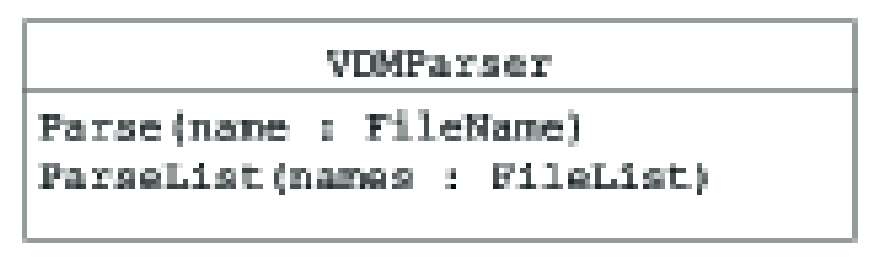
\includegraphics{VDMParser}}
%\caption{The {\tt VDMParser} interface.}\label{fig:VDMParser}
%\end{center}
%\end{figure}

\begin{figure}[tbh]
\begin{center}
\begin{tabular}{|l|}
\hline
{\tt ToolboxAPI::VDMParser } \\
\hline
{\tt Parse(in FileName name) } \\
{\tt ParseList(in FileList names) } \\
\hline
\end{tabular}
\caption{{\tt VDMParser} インターフェイス}\label{fig:VDMParser}
\end{center}
\end{figure}

{\tt \VDMParser}インターフェイスを図~\ref{fig:VDMParser}に示す。
このインターフェイスを用いて、 単一ファイルまたは一連のファイル群に対してVDM Toolbox 構文解析を行うことができる。
後者の一連のファイル群は、手作業で一覧を構築する代わりに、\texttt{\hyperlink{method.VDMProject::GetFiles}{VDMProject::GetFiles}}の呼び出しを行うことで通常は得られる。

ファイルの構文解析中にエラーが起きる場合は、検出されたエラーを記述する詳細情報を得るために続けて {\tt  \VDMErrors} インターフェイス (第~\ref{VDMErrors}章参照) に問い合わせを行うことができる。

型チェックツール、コード生成ツール、清書印刷ツール ({\tt \VDMCodeGenerator}、{\tt \VDMTypeChecker}、{\tt \VDMPrettyPrinter})に対するインターフェイスの構造は{\tt \VDMParser}と非常によく似ているが、唯一の違いは、これらのインターフェイスはクライアントが読み込み修正できるたくさんの種々の属性を持つということだ。
この属性の設定は、特定のインターフェイスの機能を制御する。
これらの3つのインターフェイスについてはここでは詳しく述べないが、個々の属性の更なる詳細と説明は第~\ref{refguide}章のIDL記述を参照とする。

\subsubsection{VDMInterpreter}

%\begin{figure}[tbh]
%\begin{center}
%\mbox{}
%\resizebox{13cm}{!}{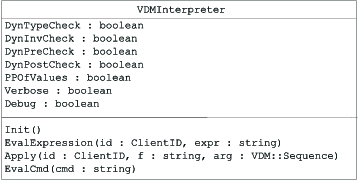
\includegraphics{VDMInterpreter}}
%\caption{The {\tt VDMInterpreter} interface.}\label{fig:VDMInterpreter}
%\end{center}
%\end{figure}

\begin{figure}[tbh]
\begin{center}
\begin{tabular}{|l|}
\hline
{\tt ToolboxAPI::VDMInterpreter } \\
\hline
{\tt DynTypeCheck: boolean } \\
{\tt DynInvCheck: boolean } \\
{\tt DynPreCheck: boolean } \\
{\tt DynPostCheck: boolean } \\
{\tt PPOfValues: boolean } \\
{\tt Verbose: boolean } \\
{\tt Debug: boolean } \\
\hline
{\tt Initialize () } \\
{\tt EvalExpression (in VDM::ClientID id, in string expr) } \\
{\tt Apply (in VDM::ClientID id, in string f, in VDM::VDMSequence arg) } \\
{\tt EvalCmd (in string cmd) } \\
{\tt SetBreakPointByPos (in string file, in long line, in long col) } \\
{\tt SetBreakPointByName (in string mod, in string func) } \\
{\tt DeleteBreakPoint (in long num) } \\
{\tt StartDebugging (in VDM::ClientID id, in string expr) } \\
{\tt VDM::VDMTuple DebugStep (in VDM::ClientID id) } \\
{\tt VDM::VDMTuple DebugStepIn (in VDM::ClientID id) } \\
{\tt VDM::VDMTuple DebugSingleStep (in VDM::ClientID id) } \\
{\tt VDM::VDMTuple DebugContinue (in VDM::ClientID id) } \\
\hline
\end{tabular}
\caption{{\tt VDMInterpreter} インターフェイス}\label{fig:VDMInterpreter}
\end{center}
\end{figure}

 {\tt \VDMInterpreter} インターフェイスを図~\ref{fig:VDMInterpreter}に示す。
このインターフェイスはインタープリタを使用して、VDM式の評価とデバッグをし、仕様中の関数や演算を起動する。
{\tt EvalExpression(client\_id, expr)}を呼び出すと、文字列引数である {\em expr} 内の式が評価され、クライアントに結果が返される。
結果は、第~\ref{idldescriptionvalues} 章に述べるVDM 値 {\tt \Generic} として表される。
たとえば、

\newpage
\begin{quote}
\begin{verbatim}    
EvalExpression(client_id, "[e | e in set {1,...,20} 
             & exists1 x in set {2,...,e} & e mod x = 0 ] ")
\end{verbatim}
\end{quote}

これは、1から20の間のすべての素数からなる列をもった {\tt \Generic} を返す。列からすべての素数を抽出するかわりに、(VDMにおいては)より効率的な関数である{\tt Primes}を指定し、インターフェイスの{\tt Apply} メソッドを通して発動することもできる:

\begin{quote}
\begin{verbatim}    
Apply(client_id, "Primes", s)
\end{verbatim}
\end{quote}

ここでの {\tt s} は関数の引数である。
{\tt Apply} もまたある{\tt \Generic}に含まれる VDM値と同様に、与えられた引数に対して関数を適用した結果を戻す。
(この例題は、{\tt Apply}を用いたときの関数に対して引数をどのように渡すかについて、実際には多少単純化している。)
 {\tt Apply} の正確な使用法は、 C++ クライアントに対しては第~\ref{cpp:interp}章に、Java クライアントに対しては第~\ref{java:interp}章に、述べる。

この例題では、整数列の構築にインタープリタ利用が便利である:

\begin{quote}
\begin{verbatim}    
s = EvalExpression(client_id, "[e|e in set {1,...,20}]")
\end{verbatim}
\end{quote}

さらに戻り値 {\tt s} を {\tt  Apply}の引数として用いる。 
この代わりに、手作業で列を構築することも可能ではある。

すでに言及した関数とは別に、インタープリタインターフェイスはクライアントから修正が可能なたくさんの属性(ブール値)をもつ。
これら属性の設定がインタープリタの動作を制御する。
最初の5つの属性 ({\tt DynTypeCheck},{\tt DynInvTheck}, {\tt DynPreCheck}, {\tt DynPostCheck}, {\tt  PPOfValues}) は、このインタープリタのオプションに相当し、VDM Toolboxのユーザーインターフェイスから設定が可能である。
これらは、不変数、事前条件、事後条件等の動的な型チェックといった場面の制御を行う。
残る2つの属性、 {\tt Verbose} と{\tt Debug}は、API がインタープリタを使用する方法を制御する。
{\tt Verbose}は、インタープリタを使用した結果をそのままVDM Toolboxのユーザーインターフェイスに反映すべきかどうか、の制御を行う。
 {\tt Verbose} が偽であれば、ユーザーインターフェイスに結果を反映させることなしに、クライアントはインタープリタを ``silently" に使用することになる。
 {\tt Debug}属性は、仕様のブレイクポイントが評価中に生かされるかどうかを制御する。
 {\tt Debug} が真と設定されていれば、評価はそれぞれのブレイクポイントで一時停止し、ユーザーは仕様をデバッグできる。
この場合、 {\tt Apply} や {\tt  EvalExpression}への呼び出しは、ユーザーのデバッグ終了までは戻らない。

{\tt SetBreakPointByPos}と {\tt SetBreakPointByName}のメソッドを用いて、ブレイクポイントを設定することができる。
先のメソッドはファイルと位置 (行、列) を引数にとる一方、後者はモジュール名称と関数名称を求める。
両メソッド共に設定されたブレイクポイントの数を返す。
この数はブレイクポイントを削除するときに再び利用できる({\tt DeleteBreakPoint})。
デバッグはその後の {\tt StartDebugging}の呼び出しで始まる。
このメソッドは引数に {\tt ClientID} と式(列) をとる。
{\tt StartDebugging}は、評価が終了するかブレイクポイントに出会うと戻る。
 {\tt VDMTuple}を戻すが、評価状態 ({\tt <BREAKPOINT>}、 {\tt <INTERRUPT>}、 {\tt <SUCCESS>} 、 {\tt <ERROR>}のいずれか) と、 {\tt <SUCCESS>}の場合ならば MetaIV 値となる評価結果が含まれる。
 {\tt DebugStep}、 {\tt DebugStepIn}、 {\tt DebugSingleStep}、{\tt DebugContinue} のメソッドは仕様を通して用いることができる。

2つの関数を含むモジュール \texttt{A} を仮定する:

\begin{verbatim}
module A
  ...
  functions
     foo: nat -> nat
     foo (a) == a + 1;

     bar: nat -> nat
     bar (b) = foo (b)
  ...
\end{verbatim}

関数 {\tt foo}に対してブレイクポイントを設定するために、 {\tt SetBreakPointByName ("A", "foo")} を用いることもできる。
{\tt StartDebugging (id, "A`bar(1))} の呼び出しはその後、{\tt bar}における{\tt foo (b)} の呼び出しに出会った後に戻される。
結果は {\tt mk\_( <BREAKPOINT>,<<UNDEFINED>> )}となるである。
 {\tt DebugContinue}の呼び出しは評価を続け、 {\tt mk\_( <SUCCESS>, 2 )}が返されるであろう。

\subsubsection{VDMErrors}
\label{VDMErrors}

%\begin{figure}[tbh]
%\begin{center}
%\mbox{}
%\resizebox{8cm}{!}{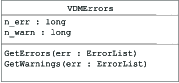
\includegraphics{VDMErrors}}
%\caption{The {\tt VDMErrors} interface.}\label{fig:VDMErrors}
%\end{center}
%\end{figure}

\begin{figure}[tbh]
\begin{center}
\begin{tabular}{|l|}
\hline
{\tt ToolboxAPI::VDMErrors } \\
\hline
{\tt NumErr: short } \\
{\tt NumWarn: short } \\
\hline
{\tt GetErrors(out ErrorList err) } \\
{\tt GetWarnings(out ErrorList err) } \\
\hline
\end{tabular}
\caption{{\tt VDMErrors} インターフェイス}\label{fig:VDMErrors}
\end{center}
\end{figure}

 {\tt \VDMErrors} インターフェイスを図~\ref{fig:VDMErrors}に示す。
このインターフェイスの状態は、構文解析、型チェック、コード生成、清書、の最中にエラーが起きた場合に、更新される。
属性{\tt n\_err}と {\tt n\_warn}を通してエラーと警告の数を求めるためには、このインターフェイスを使おう。
この2つのメソッドが、詳細な情報を得るためのエラーや警告の列を返す。

\subsection{VDM値のIDL記述}
\label{idldescriptionvalues}

 VDM Toolboxのインターフェイスの説明を行ったので、次はどのようにVDM値がAPIを通りぬけるか、つまりどのようにして VDM 値は VDM Toolboxからクライアントに渡されるのか、また逆はどうかといったことに話を移す。

与えられている例題コードは C++で記述されている。
Java構文については第~\ref{writingajavaclient} 章を参照する。

すでに述べたが、 {\tt  \VDMInterpreter}インターフェイスの {\tt EvalExpression} メソッドは評価の結果を1つのVDM 値として返し、 {\tt Apply} メソッドは、関数または操作に対する引数の一覧と同じように、VDM値のVDMの列を引数とする。
このようなVDM値を操作する方法については第~\ref{ref:vdmapi}章に記述されていて、IDL ファイルである {\tt metaiv\_idl.idl}にも記されている。
 IDL インターフェイスの構造は、VDM C++ Library の構造に( \cite{LibMan-SCSK}に記されているとおり)可能な限り近づけてある。
VDM C++ ライブラリの各々のクラスは、 IDL 記述中の1つのインターフェイス(同じ名前のもの) に一致する。 
図~\ref{fig:VDMvalues} では、すべての具体的なVDM値が同じスーパークラス{\tt  \Generic}から継承されているという事実が描かれる。
図では有効なVDM値のほんの一部だけが示されているということに注意を与えておこう。

\begin{figure}[tbh]
\begin{center}
\mbox{}
\resizebox{14cm}{!}{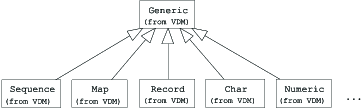
\includegraphics{VDMvalues}}
\caption{VDM 値の継承構造}\label{fig:VDMvalues}
\end{center}
\end{figure}

以下は、インタープリタより返されたVDM値の内容をどう読み込むかの例題である:

\begin{verbatim}
01  VDM::VDMGeneric_var g;
02  g = interp->EvalExpression(client_id, 
                            "{ e |-> 2**e | e in set {1,...,16}}");
03  if(!g->IsMap()){
04    // エラーを示す...
05    ...
06  }
07  else{
08    VDM::VDMMap_var m;
09    m = VDM::VDMMap::_narrow(g);
10    VDM::VDMGeneric_var iter;
11    for(int i = m->First(iter); i; i = m->Next(iter)){
12      VDM::VDMGeneric_var rng = m->Apply(client_id, iter);
13      cout << iter->ToAscii() << "-->" << rng->ToAscii() << "\n"; 
14      iter->Destroy();
15      rng->Destroy();
16    }
17  }
18  g->Destroy();
\end{verbatim}

インタープリタは {\tt  \VDMGeneric}における評価結果を返す。
このため、変数 {\tt g} は {\tt  VDM::Generic\_var}\footnote{クライアントで使用される特別な {\tt \_var} 型の記述、また CORBA オブジェクト参照の使用、について第 ~\ref{writingacppclient} 章を参照のこと。} として宣言され、クライアントで使用される特別な {\tt \_var} 型の記述に対して {\tt EvalExpression} からの結果保持のために用いられる。 
インタープリタで評価される式は写像内包であり; したがって {\tt g} に含まれる
値は  {\tt \Map}型であるとすべきであろう。
 {\tt \Generic} インターフェイスの {\tt IsMap} メソッドは、これが本当に3行目に示されるような場合であるのかをチェックするために用いることができる。
 {\tt g} が {\tt \Map} 型でなければエラー信号が伝えられる。
そうでない場合 {\Generic}の {\Map} 型への変換はうまくいく。
オブジェクト参照をキャスト (またはnarrow) するには、 ORB 実装により供給された{\tt \_narrow} メソッドを用いる。 
 9行目で{\tt \VDMGeneric} から {\tt \VDMMap}へ制限する方法を示す。
{\tt \VDMMap} 型のオブジェクト参照である {\tt m}と共に、 {\Map}インターフェイスのすべてのメソッドが現在利用可能である。
{\tt First} と {\tt Next}を用いることで、マップ ( 11行目)の定義域を通しての繰り返しが可能であり、 {\tt Apply} ( 12行目)を用いればマップ中のキーとなる値を取り出すことができる。
これらのメソッドへの同時アクセスは \emph{one} クライアントのみとすべき、と覚えておきたい。
同時に使用したクライアントは、 {\tt VDMMap}に含まれる全値を得ることができないかもしれない。

VDM 値の印刷を提供するため、 {\Generic} インターフェイスは (したがって他のすべてのVDM 値は) VDM値のASCII表現を返す {\tt ascii} メソッドを準備している。
13 行目で、このメソッドがマップ {\tt m}の各要素の印刷に用いられる。

まとめ: この簡単な例題で、インタープリタを用いてマップを構築するが、このマップを通して繰り返すための{\tt \VDMMap}のさまざまなメソッドを使用して連続して印刷が行われる。
上記の例題の出力は次の通り: 

\begin{quote}
\begin{verbatim}    
1-->2 
2-->4 
3-->8 
... (短縮のため行を削除) ...  
16-->65536
\end{verbatim}
\end{quote}

\subsubsection{分散オブジェクトとしてのVDM値}

VDM 値がサーバーからクライアントに渡されるとき、常にサーバー内の分散オブジェクトの``ハンドル" あるいはオブジェクト参照として渡される。
つまり、クライアントに使用される実際の VDM 値は、実は VDM Toolbox によって操作されたサーバーのアドレス空間に含まれるものである。
こうした理由から、クライアントが保持する {\em すべての} VDM 値は、クライアントが値をもう使用しないというときにはサーバー中で明示的に解放されなければならない。
クライアントはVDM値の {\tt Destroy} メソッドを呼び出すことでこれを行う。
 上記例題の14から 15行目で、{\tt m}の定義域の各要素を表すのに用いられたオブジェクト{\tt iter}と 、{\tt m}の値域の相当する要素を保持するために用いられた {\tt rng}は、破棄される。
最後に、18行目でインタープリタにより生成された VDM 値 {\tt g}は破棄される。
クライアントが値をもう必要としなくなったとき、この方法で破棄がなされないとしたら、 その後にVDM Toolboxで破棄されることはない。 
この結果、VDM Toolbox処理ではメモリー使用量が増大する。

そのオブジェクトに対して{\tt Destroy}メソッドを呼ぶといった明白なオブジェクト破棄の代わりに、{\tt PushTag} と {\tt  DestroyTag}という{\tt \VDMApplication} インターフェイスの2つのメソッドを用いる方法がある。
 {\tt PushTag} を呼ぶとタグを1つ生成するのでそれを内部タグスタックに押し込む。
タグスタック最上位のタグが、VDM Toolboxで連続して作成される全オブジェクトのタグ付けに用いられる。
 {\tt DestroyTag}を呼び出すたびにタグスタック最上位のタグが取り出されて、この値でタグ付けされた各オブジェクトに対して破棄の呼び出しがなされる。
結果として、{\tt PushTag} に対する最後の呼び出しで生成されたすべてのオブジェクトは破棄される。
 {\tt PushTag} と{\tt DestroyTag}の組み合わせを用いることで、前の例題は次のように読める:

\begin{verbatim}
01  app->PushTag(client_id);
02  VDM::VDMGeneric_var g;
03  g = interp->EvalExpression(client_id, 
                            "{ e |-> 2**e | e in set {1,...,16}}");
04  if(!g->IsMap()){
05    // エラーを示す...
06    ...
07  }
08  else{
09    VDM::VDMMap_var m;
10    m = VDM::VDMMap::_narrow(g);
12    VDM::VDMGeneric_var iter;
12    for(int i = m->First(iter); i; i = m->Next(iter)){
13      VDM::VDMGeneric_var rng = m->Apply(client_id, iter);
14      cout << iter->ToAscii() << "-->" << rng->ToAscii() << "\n"; 
15    }
16  }
17  app->DestroyTag(client_id); 
                 // 最後のPushTag()以降に生成された全オブジェクトが
                 // ここで破棄される。
\end{verbatim}

 {\tt PushTag} と{\tt DestroyTag}に対する呼び出しは、任意の深さの入れ子にされて
{\tt DestroyTag}呼び出しの全数が {\tt PushTag}の呼び出しの全数を超えない限りは、任意の深さの入れ子にできることは覚えておきたい。

\subsubsection{インタープリタから戻ってきた値の利用}

上記の例題では、インタープリタによって生成されたマップの定義域と値域を印刷するために {\tt ToAscii} メソッドを用いた。
ASCII表現に対するものとして、 {\tt  GetValue}メソッドを通しての値が利用できる。
たとえば以下のコードでは、列の要素1つ1つを二乗して結果を印刷出力する:

\begin{verbatim}
01  app->PushTag(client_id);
02  g = interp->EvalExpression(client_id, 
                               "[ e | e in set {1,...,10}]");
03  if(!g->IsSequence()){
04    exit(-1);
05  }
06  else{
07    VDM::VDMSequence_var s = VDM::VDMSequence::_narrow(g);
08    for(int i = 1; i <= s->Length(); i++){
09      VDM::VDMGeneric_var e = s->Index(i);
10      if(e->IsNumeric()){
11        VDM::VDMNumeric_var ii = VDM::VDMNumeric::_narrow(e);
12        cout << ii->GetValue() * ii->GetValue() << " ";
13      }
14    }
15  }
16  app->DestroyTag(client_id);
\end{verbatim}

この例題でも {\tt PushTag} と {\tt DestroyTag} のメソッドが用いられているが、クライアントにより使用された値はクライアントがもうそれらを必要としなくなったときにVDM Toolbox の中で解放される、ことが確実に遂行されるためであることに注意しよう。
これ以降は、すべてのコード例が {\tt PushTag} と {\tt DestroyTag}の呼び出しで ``wrapped"であると仮定し、明示的に {\tt Destroy} を呼び出すことはしない。

\subsubsection{クライアントの VDM値構築}

これまで用いてきたVDM 値は、すべてインタープリタが生成しクライアントへ返したものであった。
しかしながら、クライアントは{\tt \VDMFactory} インターフェイスを用いれば VDM値を直接構築できる。
以下の例題では、{\tt \VDMFactory}インターフェイスに対するハンドルを獲得して数値集合を構築する:

\begin{verbatim}
VDM::VDMFactory_var fact = app->GetVDMFactory();
VDM::VDMSet_var s = fact->MkSet(client_id);
VDM::VDMNumeric_var elem;
for(int j=0; j<20; j++){
  elem = fact->MkNumeric(client_id, j);
  s->Insert(elem);
}
\end{verbatim}

この集合に挿入される各数値と同様に、factory interfaceが集合全体の構築に用いられることを覚えておこう。
さらにfactoryで構築された各数値は、集合に挿入された後に破棄されることも覚えておきたい。なぜならこれら要素は{\tt \VDMSequence}、 {\tt  \VDMSet}、 {\tt \VDMMap}、 {\tt \VDMRecord} 、 {\tt \VDMTuple}といった合成型に挿入されるとき、暗黙にコピーされて用いられるからである。

\subsubsection{分散されたVDM値の ``実数型" VDM C++ 値への変換 }

クライアントはインタープリタからいつVDM値を受け取るのかに留意することが重要であり、これは単にVDM Toolbox内のVDM値に対するハンドルを保持するということである。
クライアントがVDM値に対するメソッドを1つ発動するたび、この呼び出しがVDM Toolboxに分散されたVDM値に対しての仲介となる。
こういった理由から、たとえばクライアントがインタープリタから戻された長い列に対して繰り返し処理を行う場合、 VDM Toolbox は列中の要素ごとに呼び出されている。
もちろんこの方法が特別に効率的だということではない。
クライアントに保持されるVDM値に対してより効率的なアクセスを行うために、\texttt{corba\_client.h}ファイル中に宣言された{\tt GetCPPValue}関数を用いることができる。この関数は分散された VDM 値を バイト構成のIDL列に変換するものであり、もし{\tt metaiv.h}を含めて VDMライブラリである\cite{LibMan-SCSK}とリンクするならば、順番に正しい VDM C++ 値に変換されることが可能だ。
使いやすさを優先すれば、分散されたVDM値から VDM C++値への変換は{\tt corba\_client.h}で利用できる。
単に{\tt GetCPPValue}を呼び出し、それを引数として変換したいと望むオブジェクト参照に渡せばよい:

\begin{verbatim}
#include "metaiv.h"

g = interp->EvalExpression(client_id, "[ e | e in set {1,...,10}]");
Generic cpp_g;  // 一般的なC++値 cpp_g = GetCPPValue(g);
// ここで C++ 値である cpp_g はクライアントプロセスに局所的であり、
// 効率的なアクセスが行える。
\end{verbatim}

 VDM C++ 値からオブジェクト参照への変換は、関数 {\tt FromCPPValue}を通して可能であり、これは記述と同様{\tt corba\_client.h}に宣言もなされている。

Java クライアントは上記の変換を手作業で行う必要があり、クライアント \cite{CGJavaManPP-SCSK}のコンパイルおよび実行時には、クラスパスにVDM Javaライブラリを含めなければならない。
例題として、付録~\ref{A4}の Java プログラムに含まれる関数 \texttt{EchoPrimes2} を参照しよう。

\subsection{例外の取り扱い}
\label{handlingofexceptions}

IDL インターフェイスである {\tt metaiv\_idl.idl} では、CORBAの2つの例外{\tt APIError} と {\tt VDMError}を宣言する。
この2種の例外は、サーバー処理で何か具合の悪いことが起きた場合に、クライアント処理に信号を送るために用いられる。
 {\tt VDMError}がVDM値使用中のエラー信号伝達に専念する一方で、{\tt APIError} はVDM ToolboxのAPI ({\tt  corba\_api.idl})の使用中に起きるかもしれないエラー信号伝達に用いられる。
 {\tt APIError} の内容は何が失敗したかを記述する簡単なメッセージ文字列であるが、 {\tt VDMError}はエラーを示す整数を保持する。
この整数の意味は第~\ref{ref:exceptions}章で示す。

付録~\ref{A3} と ~\ref{A4} の例題では、C++とJavaそれぞれの標準的な例外の取り扱いを利用し、クライアントがこのような例外をどう取り扱うことができるかを示す。

\newpage
\section{ C++ クライアントの記述}
\label{writingacppclient}

ここでは、WindowsまたはLinux上で C++ を使ってクライアントを記述する方法について述べよう。

\subsection{CORBA 実装の選択}

この例題で使用するCORBA 実装 は CORBA 2 準拠 ORB {\em omniORB3}である。
実装は {\em AT\&T ケンブリッジ研究所}により開発されたもので、 GNU一般公有使用許諾の条件や状況下において自由に利用できる。
IDLからC++への完全マッピングを実装するomniORB3によって、いくつかのプラットフォームと C++コンパイラがサポートされている。  
ORB は以下のサイトからダウンロードできる:

\begin{quote}
\begin{verbatim}    
http://www.uk.research.att.com/omniORB/omniORB.html
\end{verbatim}
\end{quote}

またWindows 2000/XP/VistaやLinux 2.4または2.6を含む様々な手近のプラットフォームに対しては、C++の純粋ソースコードやプレコンパイルされたものが利用できる。
特殊なプラットフォームで分散物が利用できない場合は、ソースコードをダウンロードすることで実行ファイルやライブラリ類を構築することが可能である。

クライアントの実装のためには、Win32かLinuxのどちらか向けの onmiORB3 配布をダウンロードし(圧縮を解凍して)インストールしなければならない。
omniORB をインストールしたら、すぐにシステムパスの環境変数にomniORBのバイナリーディレクトリへの絶対パスを追加すべきである。
このディレクトリは様々な CORBAツール(実体のための IDLコンパイラ)を含む。
Windows向けには、実行時のクライアント実装に用いられるライブラリ群も含まれている。
プリコンパイルされた配布をダウンロードする場合なら、必要なものはこれですべてである。
これ以外の場合は、配布されたもののコンパイルを成功させるためにomniORB のインストール取扱説明書を参考にする必要がある。

omniORBの代用としては、たとえば {\em オブジェクト指向構想}による{\em Orbacus} や Sun's Java IDLからの {\em idlj} である。
 OMG CORBA 2.x 仕様やIIOP を実装するORBであればどのようなものであれ、 VDM Toolbox APIと互換性をもつべきであるが、今までこのような検査はなされていない。

Orbacus は IDL からJavaやC++ への完全なマッピングを 実装しているため、この ORB はクライアントをJavaで記述したい場合に1つの選択肢となる。

\begin{quote}
\begin{verbatim}    
http://www.ooc.com/ob/ 
\end{verbatim}
\end{quote}


Java IDL comes with an IDL to Java compiler and is available
at
Java IDL は 1つのIDL と共に Java コンパイラとなり、次で利用可能である

\begin{quote}
\begin{verbatim}    
http://java.sun.com 
\end{verbatim}
\end{quote}

しかしながら、VDM Toolboxと共に配布されるクライアント例題(付録~\ref{A3}に一覧がある)はomniORB3に特有であるため、 OmniBroker が用いられるのであればクライアント例題の多少の修正が必要である。

\subsection{クライアントの実装}

この章では、C++で記述されたクライアントからVDM Toolboxを使用する例題を通して、詳細を見ていこう。
以下は完全な例題からの抜粋であり、付録~\ref{A3}で全体を見ることができる。

\subsubsection{CORBA サービスの初期化}

クライアントから VDM Toolbox のアクセスを可能とするためには、基礎となるCORBA 実装の初期化がまずなされる必要がある。
様々なCORBA実装は必ずしも同じように初期化されるわけではないため、ここで述べる CORBA 初期化は omniORBに限ったものであることに注意して欲しい。
主なアプリケーションオブジェクトの初期化と獲得は、簡単に利用するため {\tt  corba\_client.cc} に実装されていて、 {\tt corba\_client.h}をクライアント実装に含むことで利用可能となる。
異なる CORBA 実装上のクライアントを実装したいと望むのであれば、 {\tt corba\_client.cc}の内容を移植することはそれほど難しくはないであろう。 
VDM Toolbox配布の\texttt{api/corba} サブディレクトリ中に、\texttt{corba\_client.cc} と \texttt{corba\_client.h} が見つけられるはずである。

CORBA サービスの初期化に必要なすべては次の通りである:

\begin{verbatim}
#include "corba_client.h"

main(int argc, char *argv[])
{
  init_corba(argc, argv);
  ...
}
\end{verbatim}

\subsubsection{アプリケーションオブジェクトの獲得}

VDMApplication CORBA オブジェクトに対するCORBA-参照を保持するため、もっとも簡単な方法は {\tt get\_app} メソッドを用いることで、上記の \texttt{corba\_client.h} ファイルに見つけることができる。
実装は omniORB-特化であるため、任意のORBに対しては動かない可能性がある。
そのため、COS NamingServiceと文字列化参照によるサポートも行われる。

COS NamingService とは標準化された CORBA オブジェクトサービスで、オブジェクトの実体とその名称を扱うために用いられる。
これはCORBA オブジェクトに対して、ディレクトリ階層に保存された名称をマップする。文字列化されたオブジェクト参照と違い、クライアントはたとえ VDM Toolboxとファイルシステムを共有していなくともオブジェクトに対してアクセスが可能である。
したがってこれを用いることで柔軟性が得られる。
オブジェクト管理グループ (\texttt{http://www.omg.org)}により、使用が推奨されているものである。

COS NamingServiceとCORBAオブジェクトサービスについてのより詳しい情報は、OMG CORBA ホームページ上にある(\texttt{http://www.corba.org})。

VDM-SL あるいは VDM++-Toolboxを始動するとき、 COS NameService が動作しているかどうかチェックされる。
ORB は設定ファイルを探そうとする。
設定ファイルの配置場所は、 {\tt OMNIORB\_CONFIG} 環境変数 (Windowsを使用している場合にはレジストリの対処について omniORB-説明書 を参照)を用いて指定できる。
典型的な {\tt omniORB.cfg} ファイルとして、以下のエントリーを含む:

\begin{verbatim}
ORBInitialHost gandalf
ORBInitialPort 2809
\end{verbatim}

これはポート2809の {\tt gandalf} というホスト上で、NamingService が動作していることを意味している。

omniORB はこのようなNameService (omniORB-配布の一部として \texttt{omniNames}という名の実行形式が含まれるはずである)を提供するが、事実上 \texttt{omniORB.cfg} ファイルを用いてomniORBに情報を与えているという限りにおいて、他の CORBA-準拠 NameService の使用も可能である。
更なる詳細についてはomniORB 説明書を参照のこと。
 VDM-SL Toolbox は、 {\tt VDMApplication}である {\tt VDMApplication}オブジェクトを名称{\tt SL\_TOOLBOX}にバインドする一方で、VDM++ Toolbox のアプリケーションオブジェクトでは名称 {\tt PP\_TOOLBOX}が {\tt VDMApplication}として使用される。
これによりクライアントはオブジェクトを区別することが可能となり、したがって各 Toolbox 実体の同時実行に問題はない。

ただし同じ Toolboxの2実体を実行させないことに気をつけるべきで、なぜなら先に始動した {\tt VDMApplication} オブジェクトしかクライアントからアクセスできないことになるからだ。
同じ{\tt VDMApplication}オブジェクトを使用しての2クライアント以上の実行は全く問題ないが、それらは互いに影響し合うということを覚えておこう。

 VDM Toolbox に対する主導権を獲得するためのもう1つのアプローチ- {\tt VDMApplication} CORBA オブジェクト - では、クライアントに文字列化オブジェクト参照(最新のVDMToolboxで生成される)を読み込ませ、これを CORBA オブジェクト参照に変換する。
すべての ORB 実装は2つの関数 {\tt object\_to\_string} と {\tt  string\_to\_object}を実装する必要があり、これらはオブジェクト参照をコード化および非コード化するのに用いられる。
 VDM Toolbox は 、{\tt object\_to\_string} を用いてアプリケーションオブジェクトを文字列にコード化し、この文字列をファイルに書き出す。
したがってクライアントはこのファイルを読み込んだ後に、 {\tt  string\_to\_object} を用いて文字列をオブジェクト参照に変換しなければならない。
 VDM Toolbox により生成されたファイルは、VDM-SL Toolboxでは {\tt  vdmref.ior}、 VDM++ Toolboxでは {\tt vppref.ior} という名称が与えられる。
そして{\tt VDM\_OBJECT\_LOCATION} 環境変数によって指定された場所に書き込まれる。環境変数が設定されていない場合には、 VDM ToolboxがUnix上で実行されているならばユーザーのホームディレクトリ( {\tt  \$HOME}で指定されている)のルートに配置され、Windows上で実行されているならばユーザーのプロファイルディレクトリ( {\tt \%USERPROFILE\%}で指定されている)へ配置される。

クライアントからアプリケーションオブジェクトを獲得する最も簡単な方法は、{\tt corba\_client.h}に宣言されている {\tt get\_app} を用いることである。

\begin{verbatim}
main(int argc, char *argv[])
{
 ...
 /* toolType は SL_TOOLBOX か PP_TOOLBOX に設定する */
 ToolType toolType = ...;
 VDMApplication_var app;
 get_app(app, NULL, toolType);
 ...
\end{verbatim}

この関数は最初に COS NameService は動いているかどうかチェックし、さらに、{\tt VDMApplication}であれば{\tt SL\_TOOLBOX}また{\tt VDMApplication} であれば{\tt PP\_TOOLBOX} (どちらかは {\tt toolType} フラグに依存する)という名のオブジェクトが存在するかどうかをチェックする。
 NameServiceを通してこのオブジェクトを見つけることができない場合は自動的に、{\tt VDMApplication}オブジェクトへのIOR参照を含むファイルを探し出そうとする。
 {\tt get\_app} の呼び出しを行った後は、変数{\tt app} が VDM Toolboxの主ハンドルとなる。

クライアントはサーバーに対し何らかの呼び出しを行う前に、サーバー内に自身を登録しておかなければならない。
同様に、終了時には登録解除を行う必要がある。
これは {\tt \VDMApplication}クラスの {\tt Register} と{\tt Unregister}メソッドを呼び出して行う。

\begin{verbatim}
client_id = app->Register();
...
app->Unregister(client_id);
\end{verbatim}

さてこれで実行中の VDM Toolboxのサービスにアクセスできる。


\subsubsection{C++でのオブジェクト参照}
\label{objectreferences}

C++ では、IDL記述のオブジェクトインターフェイスのためのハンドルが {\em オブジェクト参照}に含まれる。
オブジェクト参照にはインターフェイス名称に {\tt \_var} をつけた名前である。
この種のオブジェクト参照は {\em オブジェクト参照変数}\footnote{オブジェクト参照にはもっと簡単な形式である、 {\tt \_ptr}オブジェクト参照、での利用もある。
オブジェクト参照の2つの型の違いの詳細は、 \cite{omniORB3} と \cite{OMG&96} で参照するものとする。
ほとんどの場合、 {\tt \_var} オブジェクト参照だけの利用で十分である。}と呼ばれる。
たとえば {\tt VDMApplication\_var} は (適切に初期化されている場合)、 サーバーの {\tt \VDMApplication}インターフェイスに対するハンドルとなる。
インターフェイスの操作は、 {\tt \_var} オブジェクト参照で矢印 ``arrow" ({\tt ->}) を用いて呼び込まれる、たとえば {\tt \VDMApplication} インターフェイス {\tt app}の {\tt GetProject}メソッドを呼び出すのには{\tt app->GetProject()} 、という具合である。

\subsubsection{最新プロジェクトの設定}

以下のコード行では、 VDM Toolboxの{\tt \VDMProject}インターフェイスに対するハンドルを獲得し、このインターフェイスの {\tt New} メソッドと {\tt AddFile} メソッドを使う。
結果として、VDM Toolbox のこのプロジェクトは単一ファイル {\tt sort.vdm}を含む構成となる。
この方法でプロジェクトに追加されるファイルは、VDM Toolbox が始動したと同じディレクトリに配置されなければならない。
そうでない場合、絶対パスの与えられたファイル名である必要がある。
クライアントが存在しないファイルを追加しようとすると、サーバーはエラーを示して{\tt APIError}型の例外処理を実行する。
これら例外処理については第~\ref{handlingofexceptions}章に記述されている。

\begin{verbatim}
VDMProject_var prj = app->GetProject();
prj->New();  // 新規プロジェクト
prj->AddFile("sort.vdm");
\end{verbatim}

\subsubsection{構文解析ツールの使用}

クライアントが構文解析ツールを使用するために、 {\tt \VDMParser}インターフェイスへのハンドルを獲得する必要があり、あるファイルを構文分析する場合はこのインターフェイスの {\tt Parse} メソッドを呼び、唯一の引数にファイル名を指定する。
たとえば

\begin{verbatim}
VDMParser_var parser = app->GetParser();
parser->Parse("sort.vdm");
\end{verbatim}

これで {\tt sort.vdm}ファイルを構文解析する。

代わりに {\tt \VDMProject} インターフェイスを用いれば、最新プロジェクトに構成されたファイルの一覧の取得や、この各ファイルの構文解析が可能となる:

\begin{verbatim}
FileList_var fl;
prj->GetFiles(fl);

for(int i=0; i<fl->length(); i++){
  cout << (char *)fl[i] << "...Parsing...";
  if(parser->Parse(fl[i]))
    cout << "done.\n";
  else
    cout << "error.\n";
}
\end{verbatim}

この例題では、APIのいくつかの重要な面を表している。
初期設定として {\tt fl} をファイル一覧と宣言し、最新プロジェクトのファイル一覧取り出しに {\tt GetFiles}を用いる。
 {\tt \FileList}型は無限の文字列列と定義され、\pageref{ref:corbatypes}ページに示される。 
結果として、ファイルの一覧である{\tt fl}は、CORBA仕様\cite{OMG&96}により提示されたIDL列のすべてのメソッドを持つ。
IDL列の長さは {\tt length}メソッドを通して入手でき、個々の要素にはC++の通常の列と同様に添え字を付けることができる。

まとめ: 上記のコード行は最新プロジェクトのファイル一覧を取り出し、その一覧を繰り返し、各項目について各ファイルを構文解析するための{\tt Parse} メソッド呼び出しを行う。
 {\tt Parse} はファイルの構文解析が成功したことを知らせるブール値を返すことに注目しよう。
ファイル一覧を繰り返すことでプロジェクトの全ファイルを構文解析する方法は、実は必要以上の複雑な作業となる。
このかわりに {\tt ParseList} メソッドを用いることができる:

\begin{verbatim}
FileList_var fl;
prj->GetFiles(fl);
parser->ParseList(fl);
\end{verbatim}

\subsubsection{型チェックツールの使用}
\label{usingthetypechecker}

型チェックツールのインターフェイスは構文解析ツールのインターフェイスと似ている。クライアントが利用したり修正したりできるたくさんの属性をもつ。 
属性の読み取りと修正は、たとえば次のように行うことができる: 

\begin{verbatim}
// DefTypeCheckの値を得る:
int dtc = tpck->DefTypeCheck();

// ExtendedTypeCheck の値を trueに設定する
tpck->ExtendedTypeCheck(true);
\end{verbatim}

もちろんここでの \texttt{tpck} は、型チェックツールインターフェイスに対する有効なハンドルである。

\subsubsection{インタープリタの利用}\label{cpp:interp}
\label{usingtheinterpreter}

以下の例題では、インタープリタに任意のVDM式を評価させるために、インタープリタインターフェイスの {\tt EvalExpression} をどのように利用できるかを示す。

\begin{verbatim}
VDMInterpreter_var interp = app->GetInterpreter();
VDM::Generic_var g;

g = interp->EvalExpression(client_id, "[e|e in set {1,...,20} & \
  exists1 x in set {2,...,e} & e mod x = 0 ]");

if(g->IsSequence())
  cout << "All primes below 20:\n" << g->ascii() << "\n";
\end{verbatim}

 {\tt EvalExpression}に渡される文字列が評価され、評価結果は {\tt VDM::Generic}における1つのVDM値として返される。これは後に {\tt Apply}呼び出しで利用される、あるいは第~\ref{idldescriptionvalues}章に記述されたVDM値のインターフェイスにより提供されるメソッド群によって、読み取り/修正を行うことができる。
行の最後にあるバックスラッシュの中に\texttt{EvalExpression}への呼び出しが置かれるが、これはC++構文の一部である。
 VDM-SL 式を含む文字列は行替え (\verb+\n+)を含まないことを示すために用いられる。
以下の例題では、VDM Toolboxにすでに読み込まれている VDM仕様の関数をどう使用するかを表す: 

\begin{verbatim}
interp->Init();
g = interp->EvalExpression(client_id, "MergeSort([6,4,9,7,3,42])");
\end{verbatim}

仕様のどんな関数でも呼び出しが行われる前に、インタープリタ初期化の確認が不可欠であることに注意しよう。

{\tt EvalExpression}の代わりとなるのが {\tt  Apply}メソッドの使用であり、これは引数として適用する関数または操作の名称をあて、関数やメソッドに対しては引数の列をあてる。
以下の例題では{\tt MergeSort}を用いてソートされた整数の VDM 列を生成する:

\begin{verbatim}
VDMFactory_var fact = app->GetVDMFactory();
    
VDM::Sequence_var list = fact->MkSequence(client_id);
VDM::Int_var elem;
for(int j=0; j<20; j++){
  elem = fact->MkInt(client_id, j);
  list->ImpPrepend(elem);
}
\end{verbatim}

結果の列は {\tt list}となり、整数 19から減じて 0までを含む。 
 {\tt \VDMFactory} インターフェイスの使用によって、クライアント側でVDM値がどう構築されるか注意しよう。

{\tt Apply} を通して {\tt MergeSort} を呼び出すために、引数の一覧を構築しなければならない。
{\tt Apply}を通して呼び出される関数に対する引数は、  {\tt  \VDMSequence}に含まれる。
呼び出したい関数は唯1つの引数をとり、それは構築したばかりの整数の列である:

\begin{verbatim}
VDM::Sequence_var arg_l = fact->MkSequence(client_id);
arg_l->ImpAppend(list);
\end{verbatim}

ここで \texttt{MergeSort} は以下のように適用される:

\begin{verbatim}
g = interp->Apply(client_id, "MergeSort", arg_l);
\end{verbatim}

もちろんここでのインタープリタは、すでに初期化されていなければならない。
引数一覧である {\tt arg\_l} もまた factory interfaceを用いて構築される。

\subsubsection{例題に付加される解釈}

ここまでで付録~\ref{A3}の例題の大半を取り上げた。
さらにこの例題で対象としているのは、エラーの詳細情報がAPIを通してどのように検索できるか、どのように個々のモジュール状態の追加情報を得るか、ということである。
ここでは例題の詳細に踏みこむことはしないが、付録~\ref{A3}のソースコードやコメントと共に、更なる情報としてIDL記述のインターフェイスである{\tt \VDMErrors} と{\tt \VDMModuleRepos} を参照しよう。

\subsection{クライアントのコンパイル}

{\tt client\_example.cc}ファイルのコンパイルを成功させるために、以下の各要求が満たされなければならない: 

\begin{itemize}
\item  omniORB はうまくインストールされていなければならない。
バイナリー配布が特殊なプラットフォームで利用できないという場合には、同様にコンパイルがなされなければならない。
さらに、{\tt PATH}環境変数は omniORBのバイナリーディレクトリを指定していることが必要である。
\item 
 \texttt{\$TOOLBOX/api/corba}に以下のファイルが、存在していなければならない ( ここで\texttt{\$TOOLBOX} は、Toolboxがインストールされたディレクトリを表している)。
\begin{itemize}
\item {\tt client\_example.cc}
\item {\tt corba\_client.h}, {\tt corba\_client.cc}
\item {\tt corba\_api.idl}, {\tt metaiv\_idl.idl}
\item {\tt Makefile}, {\tt Makefile.nm}
\end{itemize}
\item
 VDM Toolbox には VDM C++ ライブラリ、つまりインクルードファイル {\tt metaiv.h} と、ライブラリ {\tt libvdm.a} (Unix) または {\tt
vdm.lib} (Windows)、が含まれる必要がある。 
\end{itemize}

例題をコンパイルするため、簡単にMakefileが利用できる。
 Linux では{\tt Makefile}と共に {\tt make}を実行させ、 Windowsでは {\tt Makefile.nm}と共に {\tt nmake} を用いる。
omniORB と VDM Toolboxのそれぞれのインストールディレクトリを指定するため、makeファイルのマクロ {\tt OMNIDIR} と {\tt TBDIR} を修正する必要がある。

win32下の Microsoft's Foundation Classes を使用したい場合は、 MFC ライブラリが静的にリンクされるべきであることを覚えておこう。

\subsubsection{サポートされるコンパイラ}

付録~\ref{A3}にあるクライアント例題は、Microsoft Windows 2000/XP/Vista上ではMicrosoft Visual C++ 2005 SP1を用いて、
Linux上ではGNU gcc 3または4を用いて、コンパイルおよびテストされている。

\subsection{クライアントの実行}

クライアント例題を実行する前に、 サーバーとして使用されるべきVDM Toolboxが実行中であることを確認しておく必要がある。
client where to look for the {\tt [vdm|vpp]ref.ior} file.
 クライアントに{\tt [vdm|vpp]ref.ior} ファイルを探すための場所を伝えるのに、{\tt  VDM\_OBJECT\_LOCATION} 環境変数を用いること。

\newpage
\section{Javaクライアントの記述}
\label{writingajavaclient}

\subsection{CORBA 実装の選択}

 Java 1.3 API には {\tt org.omg.CORBA}と呼ばれるパッケージが含まれ、OMG CORBA APIから Java プログラム言語へのマッピングを提供している。
このパッケージは {\tt ORB}クラスを含むが、プログラマが十分な機能をもつObject Request Brokerとして使用できるように実装を行ったものだ。 

以下の例題ではこの CORBA 実装を用いる。

 CORBA の実装に加えて、ユーザーはすでに述べた IDL モデル:{\tt corba\_api.idl} と {\tt  metaiv\_idl.idl}にアクセスする必要がある。
これらは Java のパッケージやクラスに翻訳されていて、クラスパスに {\tt ToolboxAPI.jar} ファイルを含めれば使用できる。
このファイルはToolbox 配布の一部であり、\verb+api/corba+ サブディレクトリに置かれている。

次の3つのパッケージが含まれる:

\begin{itemize}
\item  {\tt jp.co.csk.vdm.toolbox.api.corba.VDM}
  このパッケージは{\tt metaiv\_idl.idl} で定義されたVDM モジュールを含む。
その結果、各VDM値に対して1つの Java インターフェイスを含む。

\item {\tt jp.co.csk.vdm.toolbox.api.corba.ToolboxAPI} 
  このパッケージは{\tt corba\_api.idl}からのインターフェイスを含む。

\item {\tt jp.co.csk.vdm.toolbox.api} 
  このパッケージは{\tt ToolboxClient}というクラス1つのみを含む。
 VDM Toolbox CORBA APIを通して、クライアントアプリケーションを VDM Toolbox に接続するためのメソッドを実装する。
\end{itemize}

3つのパッケージすべては、{\em javadoc}プログラムで生成された HTML文書で説明がなされている。
 {\tt ToolboxAPI.jar} ファイルとHTML文書は、両方とも VDM Toolboxで配布される。

Java 1.3に続く CORBA 実装を使用しない場合でも、自分でIDL ファイルを Java に翻訳する必要がある。
\texttt{ToolboxAPI.jar}のファイルは {\tt idltojava}コンパイラ (Java Developer Connectionからダウンロード可能)を用いて生成される: 
\verb+http://developer.java.sun.com+. 
 Sun JDK 1.3を使用しているならば、実行可能形式の {\tt idlj} が配布に含まれている。
これがJava コンパイラに対応するSUN IDLで、 Javaのスタブとスケルトンを生成する。


\subsection{クライアントの実装}

この章では、Javaで記述されたクライアントからどのようにVDM Toolboxを使用するかを示す例題を通して、詳細を見ていこう。
以下は完全な例題からの抜粋で示すが、全体は付録~\ref{A4}で見ることができる。

\subsubsection{CORBA サービスのインポート}

クライアントプログラムは、 上記の3つのパッケージと共に{\tt org.omg.CORBA}パッケージをインポートすることから始めるとよいだろう:

\begin{verbatim}
import org.omg.CORBA.*;

import jp.co.csk.vdm.toolbox.api.ToolboxClient;
import jp.co.csk.vdm.toolbox.api.corba.ToolboxAPI.*;
import jp.co.csk.vdm.toolbox.api.corba.VDM.*;
\end{verbatim}

%Though capitalized, {\tt ToolboxAPI} and {\tt VDM} are Java packages.
%This is because of the OMG IDL to Java mapping (see \verb+http://www.omg.org+).

\subsubsection{アプリケーションオブジェクトの獲得}

 C++ 実装においてと同様に、VDM Toolboxに対するメインハンドル−{\tt \VDMApplication} CORBAオブジェクト−獲得のために用いられるアプローチは、クライアントにCOS NamingServiceからの参照を決断させるか、文字列化されたオブジェクト参照を読み込みこれをCORBAオブジェクト参照に変換するか、である。

\texttt{\VDMApplication} CORBAオブジェクトに対するCORBA-参照を簡単に手に入れるために可能性が最も高い方法として、 前述の\texttt{ToolboxClient.java} ファイルに見る {\tt getVDMApplication} メソッドの利用がある。

 VDM-SL あるいは VDM++ Toolboxを始めるとき、 COS NameService が動作しているかどうかがチェックされる。
ORB が設定ファイルを探そうとする。
このファイルの配置位置は {\tt OMNIORB\_CONFIG} 環境変数を用いて指定することができる (Windows使用の場合に、このためどのようにレジストリを使用するのかは omniORB-説明書を参照のこと)。 
典型とされる {\tt omniORB.cfg} ファイルでは、以下のエントリが含まれる:

\begin{verbatim}
ORBInitialHost gandalf
ORBInitialPort 2809
\end{verbatim}

これはポート 2809の {\tt gandalf}と呼ばれるホスト上で、 NamingService が動いていることを意味している。
omniORB はこのようなNameService (omniORB-配布の一部として、\texttt{omniNames}と呼ばれる実行形式があるはずである)を提供しているが、 \texttt{omniORB.cfg} ファイルを用いて omniORBに知らせている限りであれば他のどのようなCORBA-compliant NameServiceでも実際上用いることが可能だ。
さらに詳しくは omniORB 説明書を参照のこと。
Toolbox は、Sun JDK1.3からもまた {\tt tnameserv}-NamingServiceを用いてテストを行ってきている。
クライアントアプリケーションに対しては、 NameServiceをどこで見つけることができたかを知らせる必要が出てくるであろう。
また、これをコマンドラインパラメーター {\tt -ORBInitialPort <port> -ORBInitialHost <host>}で行うことも、直接ソースコードに相当するプロパティを設定することも、できる。

\begin{verbatim}
  Properties props = new Properties ();
  props.put ("org.omg.CORBA.ORBInitialHost", "gandalf");
  props.put ("org.omg.CORBA.ORBInitialPort", 2809);
  orb = ORB.init (args, props);
\end{verbatim}

VDM-SL Toolbox はその {\tt VDMApplication}オブジェクトに、{\tt VDMApplication}の中の{\tt SL\_TOOLBOX}という名を付け、一方でVDM++ Toolbox のアプリケーションオブジェクトには、{\tt VDMApplication}の中の {\tt PP\_TOOLBOX}という名称を用いる。
これによりクライアントはオブジェクトを区別することができるため、各 Toolbox のインスタンスを実行させることについての問題はなくなる。

以下のコードは {\tt VDMApplication}-オブジェクト をNameServiceから決定するのに用いられる:

\begin{verbatim}
  org.omg.CORBA.Object obj = 
     orb.resolve_initial_references ("NameService");
  NamingContext ctx = NamingContextHelper.narrow (obj);

  NameComponent nc = null;

  if (toolType == ToolType.SL_TOOLBOX)
     nc = new NameComponent ("SL_TOOLBOX", "VDMApplication");
  else
     nc = new NameComponent ("PP_TOOLBOX", "VDMApplication");

  NameComponent[] name = {nc};
  
  org.omg.CORBA.Object obj = // 完全修飾のクラスパスを使用しよう!
     ctx.resolve (name);
  VDMApplication app = VDMApplicationHelper.narrow (obj);
\end{verbatim}

同じToolboxの2つのインスタンスを実行させないよう気をつけるべきで、なぜなら先に始動した {\tt VDMApplication} オブジェクトしかクライアントからアクセスできないことになるからである。
同じ {\tt VDMApplication}オブジェクトを使用しての2クライアント数以上の実行は全く問題ないが、それらが互いに影響しあうということを覚えておこう。

 {\tt getVDMApplication}メソッドが NamingServiceを配置できない場合、文字列参照ファイルを使用して  {\tt VDMApplication}-参照の決定を試みる。
すべての ORB 実装では2つの関数{\tt  object\_to\_string} と {\tt string\_to\_object}を実装する必要があり、オブジェクト参照をコード化および非コード化するのに用いられる。
 VDM Toolbox は {\tt  object\_to\_string} を使用してアプリケーションオブジェクトを文字列としてエンコードし、この文字列をファイルに書き出す。
したがってクライアントはこのファイルを読み込んだ後に、 {\tt string\_to\_object} を用いて文字列をオブジェクト参照に変換しなければならない。
 VDM Toolbox により生成されたファイルは {\tt  vdmref.ior} あるいは {\tt vppref.ior}という名称が与えられ、{\tt VDM\_OBJECT\_LOCATION}環境変数によって指定された場所に書き込まれる。
環境変数が設定されていない場合に、VDM ToolboxがUnix 上で実行されているならばホームディレクトリ( {\tt  \$HOME}で指定されている)のルートに配置され、Windows上で実行されているならばユーザーのプロファイルディレクトリ( {\tt \%USERPROFILE\%}で指定されている)に配置される。

{\tt ToolboxClient}クラスの {\tt readRefFile} メソッドは、Toolboxにより生成されたこの \texttt{vdmref.ior} あるいは \texttt{vppref.ior} ファイルを読み込むために{\tt getVDMApplication} で使用される。
 {\tt Toolbox} クライアントクラスの{\tt getVDMApplication}メソッドを呼び出すことで、オブジェクト参照文字列で示された Toolbox に対して接続を構築することができる。
このメソッドは CORBA {\tt \VDMApplication} オブジェクトへのオブジェクト参照を返してくれる。

\begin{verbatim}
VDMApplication app = ToolboxClient.getVDMApplication(args,ref);
\end{verbatim}

{\tt getVDMApplication} の呼び出しの後、変数{\tt app} が VDM Toolboxに対する主ハンドルとなる。

クライアントはサーバーに向けての呼び出しを行う前に、サーバー中に自身を登録しなければならない。
同様にして、終了時には自身を登録解除しなければならない。
これは{\tt \VDMApplication} クラスの  {\tt Register} および{\tt Unregister}メソッドの呼び出しを行うことでなされる。

\begin{verbatim}
short client_id = app.Register();
...
...
app.Unregister(client_id);
\end{verbatim}

ここで、実行中のVDM Toolboxのサービスにアクセスする立場にたつ。

\subsubsection{最新プロジェクトの設定}

以下のコード行では、VDM Toolboxの {\tt \VDMProject}インターフェイスに対するハンドルを獲得して、このインターフェイスの {\tt New} および {\tt AddFile} メソッドを使用している。
その結果として VDM Toolbox のプロジェクトは唯1つのファイル {\tt sort.vdm}を含むように構成されている。
VDM Toolbox was started. 
この方法でプロジェクトに追加されるファイルは、 VDM Toolbox が始動した同じディレクトリに配置されていなければならない。
そうでない場合、ファイル名は絶対パスと共に与えられなければならない。
クライアントが存在しないファイルを追加しようとすると、サーバーはエラーを示す {\tt APIError} タイプの例外処理を実行しようとする。
例外処理については 第~\ref{handlingofexceptions}章に記述されている。

\begin{verbatim}
VDMProject prj = app.GetProject();
prj.New();
prj.AddFile("sort.vdm");
\end{verbatim}

\subsubsection{構文解析ツールの利用}

クライアントから構文解析ツールを使用するためには、 {\tt \VDMParser}インターフェイスに対するハンドルを獲得しなければならず、ファイルを構文解析するためには、そのファイル名を唯1つの引数として与えてこのインターフェイスの {\tt Parse} メソッドを呼び出すのである。つまり、

\begin{verbatim}
VDMParser parser = app.GetParser();
parser.Parse("sort.vdm");
\end{verbatim}

これでファイル {\tt sort.vdm}を構文解析する。

替わりとしてカレントプロジェクトのために構成されたファイルの一覧を得るために {\tt \VDMProject} インターフェイスを使用し、その後この一覧の各ファイルを構文解析することもできる:

\begin{verbatim}
FileListHolder fl = new FileListHolder();
int count = prj.GetFiles(fl);
String flist[] = fl.value;
                
for(int i=0; i<flist.length; i++){
   System.out.println("...Parsing" + flist[i] + "...");
   if(parser.Parse(flist[i]))
        System.out.println("done.");
   else
        System.out.println("error.");
}
\end{verbatim}

この例題では APIのいくつかの重要な面を表している。
初期処理として {\tt fl} をファイル一覧として宣言し、最新プロジェクトのファイル一覧を取り出し {\tt GetFiles}を用いる。
APIの IDL記述をみれば、 {\tt \FileList}型は無限の文字列列として定義されている。 
結果としてファイル一覧{\tt fl}は、CORBA仕様 \cite{OMG&96} により提出されたIDL列のすべてのメソッドをもつ。
 IDL 列の長さは{\tt length}メソッドを通して入手でき、個々の要素にJavaの通常の列と同様に添え字を付けることができる。

さらにこの例題で示されるように、Javaで状態を手渡す出力入出力のパラメーターに対するサポートとして、付加的な``holder"クラスの使用が必要となる。
これらのクラスは、 {\tt org.omg.CORBA}パッケージの基本IDLデータ型のすべてに対してできる上、typedefで定義する型以外の型を定義したすべての名前つきユーザーに対して生成される。

ユーザー定義のIDL 型に対しては、その型のマップ(Java)名に対して{\tt Holder}を付けることで  holder クラス名がつくられる。
各 holderクラスは パブリックな 実体要素、 {\tt value}、をもち、これは型付きの値である。

まとめ: 上記のコード行は最新プロジェクトのファイル一覧を取り出しその一覧を繰り返して、各項目について各ファイルを構文解析するための {\tt Parse}メソッド呼び出しを行う。
 {\tt Parse}は、ファイルの構文解析の成功を知らせるブール値を返すことに注目しよう。
ファイル一覧を繰り返すことでプロジェクトのファイルを構文解析する方法は、実は必要以上の複雑な作業となる。
この代わりに{\tt ParseList} メソッドを用いることができる:

\begin{verbatim}
FileListHolder fl = new FileListHolder();
int count = prj.GetFiles(fl);
String flist[] = fl.value;
parser.ParseList(flist);
\end{verbatim}

\subsubsection{型チェックツールの使用}

型チェックツールのインターフェイスは構文解析のインターフェイスと似ている。
クライアントが利用したり修正したりできるたくさんの属性をもつ。
属性の読み取りと修正はたとえば次のように行うことができる:

\begin{verbatim}
// DefTypeCheckの値を得る:
boolean dtc = tpck.DefTypeCheck();

// ExtendedTypeCheck の値を trueに設定する
tpck.ExtendedTypeCheck(true);
\end{verbatim}

もちろんここでの \texttt{tpck}は、型チェックツールインターフェイスに対する有効なハンドルである。


\subsubsection{インタープリタの利用}\label{java:interp}

以下の例題では、インタープリタに任意のVDM式を評価させるために、インタープリタインターフェイスの {\tt EvalExpression} をどのように利用できるかを示す。

\begin{verbatim}
VDMInterpreter interp = app.GetInterpreter();
Generic g;
g = interp.EvalExpression(client_id, 
        "[e|e in set {1,...,20} & \
              exists1 x in set {2,...,e} & e mod x = 0]");

if(g.IsSequence()){
     System.out.println("All primes below 20": " + g.ascii());
}
\end{verbatim}

{\tt EvalExpression} に渡される文字列が評価され、評価結果はある{\tt Generic}における1つのVDM値として返される。これは後に{\tt Apply}呼び出しで利用されたり、あるいは第~\ref{idldescriptionvalues}章で記述されたVDM値のインターフェイスにより提供されるメソッド群によって、読み取り/修正を行うことができる。

以下の例題では、VDM仕様の関数をどう使用するかを表す: 

\begin{verbatim}
interp.Init();
g = interp.EvalExpression(client_id, "MergeSort([6,4,9,7,3,42])");
\end{verbatim}

仕様のどのような関数でも呼び出しが行われる前は、インタープリタ初期化の確認が不可欠である。

{\tt EvalExpression}の代わりとなるのが {\tt  Apply}メソッドの使用であり、これは引数として適用する関数または操作の名称をあて、関数やメソッドに対しては引数の列をあてる。
以下の例題では{\tt MergeSort}を用いてソートされた整数の VDM 列を生成する:

\begin{verbatim}
VDMFactory fact = app.GetVDMFactory();
Sequence list = fact.MkSequence(client_id);
Numeric elem;
for(int j=0; j<20; j++){
    elem = fact.MkNumeric(client_id, j);
    list.ImpPrepend(elem);
}
\end{verbatim}                

結果となる列 {\tt list}は、整数19から減じて0までを含む。
 {\tt \VDMFactory} インターフェイスの使用により、クライアント側で VDM 値がどう構築されるのか注意しよう。

{\tt Apply}を通して {\tt MergeSort}を呼び出すために、引数の一覧を構築しなければならない。
{\tt Apply} を通して呼び出される関数に対する引数は、 {\tt \Sequence}に含まれる。呼び出したい関数は唯1つの引数を取るが、それは構築したばかりの整数の列である:

\begin{verbatim}
Sequence arg_l = fact.MkSequence(client_id);
arg_l.ImpAppend(list);
\end{verbatim}

ここで \texttt{MergeSort} は以下のように適用される:

\begin{verbatim}
g = interp->Apply(client_id, "MergeSort", arg_l);
\end{verbatim}

もちろんインタープリタは、すでに初期化されていなければならない。
引数一覧である{\tt arg\_l} もまた factoryインターフェイスを用いて構築されたものであることは、覚えておこう。

最後に、列の要素すべての合計を計算するために、返された列を通して繰り返しをどのように行うか示す:

\begin{verbatim}
Sequence s = SequenceHelper.narrow(g);
GenericHolder eholder = new GenericHolder();
int sum=0;
for (int ii=s.First(eholder); ii != 0; ii=s.Next(eholder)) {
  Numeric num = NumericHelper.narrow(eholder.value);
  sum = sum + (int) num.GetValue();
}
\end{verbatim}

\subsubsection{例題に追加される解釈}

ここまでで、付録~\ref{A4}の例題の大半を取り上げた。
さらにこの例題で対象としているのは、エラーの詳細情報がAPIを通してどのように検索できるか、どのように個々のモジュール状態の追加情報を得るか、ということである。
その上で、配布された VDM 値を ``実数型'' VDM Java 値に変換する方法も示す。
 ここでは例題の詳細にさらに踏み込むことはしないが、付録~\ref{A4}のソースコードやコメントと共に、更なる情報としてIDL記述のインターフェイスである {\tt \VDMErrors} と{\tt \VDMModuleRepos} を参照しよう。

\subsection{クライアントのコンパイル}

{\tt client\_example.java} ファイルは、以下のコンパイラを用いてコンパイルされなければならない:

\begin{quote}
\begin{verbatim}
jdk1.3
\end{verbatim}
\end{quote}

次のように記述することで、主プログラムのコンパイルを行うことができる:

\begin{quote}
\begin{verbatim}
javac client_example.java
\end{verbatim}  
\end{quote}

{\tt CLASSPATH} 環境変数が{\tt ToolboxAPI.jar}ファイルを含むことを確認すること。
もしUnix Bourne シェルまたは互換性のあるシェルを用いているならば、次のコマンドが利用できる:

\begin{quote}
\begin{verbatim}
CLASSPATH=ToolboxAPI_Library/ToolboxAPI.jar:$CLASSPATH
export CLASSPATH
\end{verbatim}  %$
\end{quote}

{\tt ToolboxAPI\_Library} を、 {\tt ToolboxAPI.jar}ファイルがインストールされたディレクトリ名に置きかえること。

Windowsベースのシステムで作業をしている場合は、 Windowsコマンドプロンプト内で以下のコマンドを用いることができる: 

\begin{quote}
\begin{verbatim}
set CLASSPATH=ToolboxAPI_Library/ToolboxAPI.jar;$CLASSPATH
\end{verbatim}  %$
\end{quote}

Windowsに対しては、区切り文字は``{\tt :}''ではなく ``{\tt ;}'' を使用しなければならないことに注意しよう。

\subsection{クライアントの実行}

クライアント例題を実行する前に、サーバーとして使用されるべき VDM Toolbox が実行中であることを確認しておく必要がある。

既定では、例題プログラムは Linux上でVDM-SL Toolbox と共に実行されていると仮定する。
この場合、単に次の実行をする。

\begin{quote}
\begin{verbatim}
java client_example.java
\end{verbatim}  
\end{quote}

Windows 上の実行では WIN property を設定しなければならず、 VDM++ Toolbox を用いた実行では、 VDMPP プロパティを設定しなければならない。

\begin{quote}
\begin{verbatim}
java -DVDMPP -DWIN client_example
\end{verbatim}  
\end{quote}

\newpage




\section{API 参照ガイド}\label{refguide}

\subsection{Corba API}\label{ref:corbaapi}


\subsubsection{型}\label{ref:corbatypes}

以下の型同義語が定義されている:

\begin{longtable}{|>{\pbs\raggedright\ttfamily}p{6.6cm}%
                  |>{\pbs\raggedright\ttfamily}p{6.6cm}|} \hline
  \textrm{\bfseries 名称} &  \textrm{\bfseries 同義語の対象} \\ \hline
\hyperdef{type}{ModuleName} ModuleName & string\\
\hyperdef{type}{ModuleList} ModuleList & sequence<ModuleName> \\
\hyperdef{type}{ClassName}  ClassName  & string\\
\hyperdef{type}{ClassList}  ClassList  & sequence<ClassName>\\
\hyperdef{type}{FileName}   FileName   & string\\
\hyperdef{type}{FileList}   FileList   & sequence<FileName>\\ 
\hyperdef{type}{ErrorList}  ErrorList   & sequence<{\ErrorStruct}>\\ 
\hline
\end{longtable}

以下の列挙が定義されている
\hyperdef{type}{ToolType}\mbox{}
\begin{verbatim}
  enum ToolType {SL_TOOLBOX, PP_TOOLBOX};
\end{verbatim}\label{api:ToolType}

以下の構造が定義されている:

\subsubsection{エラー構造}\label{api:ErrorStructure}
\hyperdef{struct}{Error}\mbox{}
\begin{longtable}{|>{\pbs\raggedright\ttfamily}p{6.6cm}%
                  |>{\pbs\raggedright}p{6.6cm}|} \hline
  \textrm{\bfseries 変数} &  \textrm{\bfseries 意味} \\ \hline
{\FileName} fname
  & エラー/警告の検出されたファイル名
\\ \hline
unsigned short line
  & エラー/警告の行番号
\\ \hline
unsigned short col
  & エラー/警告の列番号
\\ \hline
string msg
  & エラー/警告のテキスト
\\ \hline
\end{longtable}

\subsubsection{ModuleStatus 構造}\label{api:ModuleStatusStructure}
\hyperdef{struct}{ModuleStatus}\mbox{}
\begin{longtable}{|>{\pbs\raggedright\ttfamily}p{6.6cm}%
                  |>{\pbs\raggedright}p{6.6cm}|} \hline
  \textrm{\bfseries 変数} &  \textrm{\bfseries 意味} \\ \hline
boolean SyntaxChecked
  & モジュール(またはクラス)が構文チェック済みであるかどうかを示す属性
\\ \hline
boolean TypeChecked
  & モジュール(またはクラス)が型チェック済みであるかどうかを示す属性
\\ \hline
boolean CodeGenerated
  & モジュール(またはクラス)がコード生成済みであるかどうかを示す属性
\\ \hline
boolean PrettyPrinted
  & モジュール(またはクラス)が清書済みであるかどうかを示す属性
\\ \hline
\end{longtable}


\subsubsection{VDMApplicationインターフェイス}
\hyperdef{interface}{VDMアプリケーション}\mbox{}
\begin{interfacetable}
readonly attribute {\ToolType} Tool
  & サーバー側Toolboxに対するツールの型を返す。
\\ \hline
{\ClientID} Register()
  & unique client idを返す。クライアントは何かのAPIを実行する前にサーバー側に自身を登録するべきである。
\\ \hline
void Unregister({\ClientID} id)
  & クライアント\texttt{id}と結びついたリソースを解放する。クライアントが終了するときはこれが呼ばれるべきである。
\\ \hline
{\VDMProject} GetProject()
  & 現プロジェクトに対するハンドルを返す。
\\ \hline
{\VDMInterpreter} GetInterpreter()
  &  Toolbox インタープリタに対するハンドルを返す。
\\ \hline
{\VDMCodeGenerator} GetCodeGenerator()
  & Toolbox コード生成ツールに対するハンドルを返す。
\\ \hline
{\VDMParser} GetParser()
  & Toolbox 構文解析に対するハンドルを返す。
\\ \hline
{\VDMTypeChecker} GetTypeChecker()
  & Toolbox 型チェックツールに対するハンドルを返す。
\\ \hline
{\VDMPrettyPrinter} GetPrettyPrinter()
  & Toolbox 清書ツールに対するハンドルを返す。
\\ \hline
{\VDMErrors} GetErrorHandler()
  & Toolbox エラーインターフェイスに対するハンドルを返す。
\\ \hline
{\VDMModuleRepos} GetModuleRepos()
  & Toolbox モジュール (またはクラス) リポジトリに対するハンドルを返す。
\\ \hline
{\VDMFactory} GetVDMFactory()
  & VDM value factoryに対するハンドルを返す。 CORBA 2.x では remote object instantiationをサポートしないため、この factory がCORBA VDM オブジェクト (たとえば VDMSequence、 VDMToken\ldots)の生成のために用いられる必要がある。
\\ \hline
void PushTag(in {\ClientID} id)
  & クライアント\texttt{id}に対する unique tag を生成し、Toolboxの内部タグスタック上にこれを押し込む。このクライアントに対してToolboxで生成されたすべてのオブジェクトは、その後このタグでタグ付けされる。
\\ \hline
void DestroyTag(in {\ClientID} id) \APIError
  & \texttt{{\ClientID}}に対するタグスタック上の一番上のタグを取り出し、この値でタグ付けされたすべてのオブジェクトを破壊する。
\\ \hline
\end{interfacetable}

\subsubsection{VDMCodeGeneratorインターフェイス}
\hyperdef{interface}{VDMCodeGenerator}\mbox{}
\begin{interfacetable}
attribute boolean GeneratePosInfo
  & 位置情報の生成を有効化または無効化する。これによって生成コード中の構築物すべては仕様にまでさかのぼることを許可される。 既定は \textsf{false}。 
\\ \hline
enum LanguageType {CPP, JAVA}
  & コード生成ツールの可能な対象言語\\
\\ \hline
boolean GenerateCode(in {\ModuleName} name, in LanguageType targetLang) \APIError
  & モジュール (またはクラス) \texttt{name}に対して C++/Java コード (targetLang flagに従う) を生成する。\texttt{name} が現プロジェクト内で有効なモジュール名またはクラス名でなかった場合、またVDM-SL モジュールに対してJava コードを生成しようとした場合、例外を起こす (Java コード生成は VDM++-クラスに対してのみ利用可能なものであるから)。
\\ \hline
boolean GenerateCodeList(in {\ModuleList} names) \APIError
  & \texttt{names}中の各モジュール (またはクラス)名 に対して C++/Java コードを生成する。 \texttt{names}中の名称で現プロジェクトで有効なモジュール名やクラス名でないものがあった場合、またVDM-SL モジュールに対してJava コードを生成しようとした場合、例外を起こす。

\\ \hline
\end{interfacetable}

\subsubsection{VDMErrorsインターフェイス}
\hyperdef{interface}{VDMErrors}\mbox{}
\begin{interfacetable}
readonly attribute unsigned short NumErr
                                        & 直前の動作で
                                          生成されたエラーの数を返す。
\\ \hline
readonly attribute unsigned short NumWarn()
                                        & 直前の動作で
                                          生成された警告の数を返す。
\\ \hline
unsigned short GetErrors(out ErrorList err)  
                                        & \texttt{err}中の直前の動作で
                                          生成されたエラーの一覧を返す。
\\ \hline
unsigned short GetWarnings(out ErrorList err)
                                        & \texttt{err}中の直前の動作で
                                          生成された警告の一覧を返す。
\\ \hline
\end{interfacetable}

\subsubsection{VDMInterpreterインターフェイス}
\hyperdef{interface}{VDMInterpreter}\mbox{}
\begin{interfacetable}

attribute boolean DynTypeCheck
  & 動的型チェックを有効化または無効化する。既定は \textsf{false}。
\\ \hline
attribute boolean DynInvCheck
  & 動的不変数チェックを有効化または無効化する。既定は \textsf{false}。真の場合は、 \texttt{DynTypeCheck} 属性が自動的に真に設定される。
\\ \hline
attribute boolean DynPreCheck
  & 動的事前条件チェックを有効化または無効化する。既定は \textsf{false}。 
\\ \hline
attribute boolean DynPostCheck
  & 動的事後条件チェックを有効化または無効化する。既定は \textsf{false}。 
\\ \hline
attribute boolean PPOfValues
  & 清書機能を有効化または無効化する。既定は \textsf{true}。 
\\ \hline
attribute boolean Verbose
  & Toolboxとの冗長な対話、つまりAPIを通して実行された動作結果のインタープリタウィンドウでの繰り返し、を有効化または無効化する。既定は \textsf{false}。
\\ \hline
attribute boolean Debug
  & デバッグモードを有効化または無効化する。このモードでは仕様中のブレイクポイントが生かされる。ブレイクポイントが評価されるときは一時停止を行い、ユーザーは実際上のデバッグを行うためにグラフィカルユーザーインターフェイスと付き合う必要がある。既定は \textsf{false}。
\\ \hline
void Initialize() %\APIError
 % Technically raises an exception, but the circumstances
 % in which this occurs are not clear
  & インタープリタを初期化する。評価の前になされる必要がある。
\\ \hline
{\VDMGeneric} EvalExpression(in {\ClientID} id, in string expr) \APIError
  & ID \texttt{id} のクライアントの代わりに、 \texttt{expr}を評価する。
    評価結果はメソッドの結果として返ったものだ。 \texttt{Verbose} が
    \textsf{true}であるならば、結果はモニターに投影される。
    実行時エラーは例外を引き起こす。
\\ \hline
{\VDMGeneric} Apply(in {\ClientID} id, in string f, in {\VDMSequence} arg)
\APIError
  & クライアント\texttt{id}の代わりに、関数(または操作) \texttt{f} を引数 \texttt{arg}に適用する。 関数(または操作)呼び出しの結果は、メソッドの結果として返される。
    実行時エラーは例外を引き起こす。
\\ \hline
void EvalCmd(in string cmd) 
  & インタープリタに直接書き込まれたように、コマンド \texttt{cmd} を評価する。    
    % Note that idl file states that an exception may be raised here,
    % but this does not seem to be the case in practice.
\\ \hline
long SetBreakPointByPos(in string file, in long line, in long col) 
  & 指定ファイルの指定位置(行、列)にブレイクポイントを設定し、
    新しいブレイクポイントの数を返す。
    例外または -1 の戻り値が、エラーが起きたことを示す
    (たとえば、ファイルが存在しないまたは
    指定された行番号が有効でない場合)。
\\ \hline
long SetBreakPointByName(in string mod, in string func) \APIError
  & 指定モジュールの指定関数(func)にブレイクポイントを設定し、
  新しいブレイクポイントの数を返す。
  例外または-1の戻り値は、エラーが起きたことを示す
  (たとえばモジュールまたは関数が存在しない場合)。
\\ \hline
void DeleteBreakPoint(in long num) \APIError
  & ブレイクポイントの削除に使用される。
  ブレイクポイントで返された数を、1つのパラメーターとして、メソッドを設定する。
\\ \hline
{\VDMTuple} StartDebugging (in {\ClientID} id, in string expr) \APIError 
  & 式のデバッグを始める。式の評価が終了した場合、またはブレイクポイントに出会った場合、このメソッドが返る。
 評価状態 ( {\tt <BREAKPOINT>}、 {\tt <INTERRUPT>}、 {\tt <SUCCESS>}、 {\tt <ERROR>}、のいずれか)を含める{\tt VDMTuple}を返すことができて、 {\tt <SUCCESS>}の場合は、結果の評価を表すMetaIV値も。

\\ \hline
{\VDMTuple} DebugStep (in {\ClientID} id) \APIError 
  & このメソッドはtoolboxにおける{\tt step}コマンドと同等である。
  これは次の文を実行しその後中断する。関数や操作の呼び出しには立ち入らない。
  評価状態(
  {\tt <BREAKPOINT>}、 {\tt <INTERRUPT>}、 {\tt <SUCCESS>} 、 {\tt <ERROR>}のいずれか)
  を含む{\tt VDMTuple}を返し、
  {\tt <SUCCESS>} (これは、式がうまく評価できたことを意味する) の場合には、
   MetaIV 値として評価の結果を返す。
\\ \hline
{\VDMTuple} DebugStepIn (in {\ClientID} id) \APIError 
  & このメソッドはtoolboxにおける {\tt stepin}コマンドと同等である。
  これは次の文を実行しその後中断する。
  関数や操作の呼び出しにも立ち入る。
  評価状態 (
   {\tt <BREAKPOINT>}、 {\tt <INTERRUPT>}、 {\tt <SUCCESS>}、 {\tt <ERROR>}のいずれかになり得る)を含む{\tt VDMTuple}を返し、
{\tt <SUCCESS>}
  (これは、式がうまく評価できたことを意味する) の場合には
  MetaIV値として評価の結果を返す。
\\ \hline
{\VDMTuple} DebugSingleStep (in {\ClientID} id) \APIError 
  & このメソッドはtoolboxにおける{\tt singlestep} コマンドと同等である。
  これは次の式または文を実行しその後中断する。
  評価状態 (
   {\tt <BREAKPOINT>}、 {\tt <INTERRUPT>}、 {\tt <SUCCESS>}、{\tt <ERROR>}の
  いずれかになり得る)を含む {\tt VDMTuple} 値を返し、
  {\tt <SUCCESS>}(これは、式がうまく評価されたことを意味する) の場合は、
  MetaIV値として評価の結果を返す。
\\ \hline
{\VDMTuple} DebugContinue (in {\ClientID} id) \APIError 
  & このメソッドはtoolboxにおける{\tt cont}コマンドと同等である。
  これはブレイクポイントに出会った後の実行を継続する。
  評価状態(
  {\tt <BREAKPOINT>}、 {\tt <INTERRUPT>}、 {\tt <SUCCESS>}、{\tt <ERROR>}のいずれかになり得る)を含む {\tt VDMTuple} 値を返し、
  {\tt <SUCCESS>} (これは、式がうまく評価されたことを意味する)の場合はMetaIV 値として評価の結果を返す。
 
\\ \hline

\end{interfacetable}

\subsubsection{VDMModuleReposインターフェイス}
\hyperdef{interface}{VDMModuleRepos}\mbox{}
\begin{interfacetable}
unsigned short FilesOfModule(out {\FileList} files, in {\ModuleName} name)
 %\APIError 
 % Technically raises an exception, but the circumstances
 % in which this occurs are not clear
 & \texttt{files}の中のモジュール(またはクラス)\texttt{name}を含むファイルの名称を引き渡す。
   フラットモジュールの場合には、1つのモジュール名 \texttt{DefaultMod}はいくつものファイルに分散されているかもしれないが、
これ以外の場合、文字列はきっちり1つの名称から構成されることになる。
   ファイル数を返す。
\\ \hline
void Status(out {\ModuleStatus} state, in {\ModuleName} name) \APIError
 & \texttt{state}にモジュール(またはクラス) \texttt{name}の状態を引き渡す。
 \texttt{name}が現モジュールに存在しない場合は、例外を起こす。
\\ \hline
unsigned short SuperClasses(out {\ClassList} classes, in {\ClassName} name)
 \APIError 
 &  \texttt{name}クラスのスーパークラスの \texttt{classes}一覧に引き渡す。
    \vdmpp 仕様では、 \vdmsl toolbox で呼ばれた場合には例外を起こす。
\\ \hline
unsigned short SubClasses(out {\ClassList} classes, in {\ClassName} name)
 \APIError
 & \texttt{name}クラスのサブクラスの \texttt{classes} 一覧に引き渡す。
   \vdmpp 仕様では、 \vdmsl toolbox で呼ばれた場合には例外を起こす。
\\ \hline
unsigned short Uses(out {\ClassList} classes, in {\ClassName} name)
 \APIError
 & \texttt{name}クラスで使用されるクラスの \texttt{classes} 一覧に引き渡す。
   \vdmpp 仕様では、\vdmsl toolbox で呼ばれた場合には例外を起こす。
\\ \hline
unsigned short UsedBy(out {\ClassList} classes, in {\ClassName} name)
 \APIError
 & \texttt{name}クラスを使用するクラスの \texttt{classes} 一覧に引き渡す。
   \vdmpp 仕様では、 \vdmsl toolbox で呼ばれた場合には例外を起こす。
\\ \hline
\end{interfacetable}

\subsubsection{VDMParserインターフェイス}
\hyperdef{interface}{VDMParser}\mbox{}
\begin{interfacetable}
boolean Parse(in {\FileName} name) \APIError
  &  \texttt{name}ファイルがうまく構文解析された場合に \textsf{true} を返す
    ; それ以外は \textsf{false}を返し
    \texttt{\VDMErrors} インターフェイスの状態が修正される。
    このファイルが存在しない場合は例外を起こす。
\\ \hline
boolean ParseList(in {\FileList} names) \APIError
  &  \texttt{names} 内のファイルすべてがうまく構文解析された場合に
     \textsf{true} を返す。それ以外は \textsf{false}を返し
    \texttt{\VDMErrors} インターフェイスの状態が更新される。 
    いずれのファイルも存在しない場合は例外を起こす。
\\ \hline
\end{interfacetable}

\subsubsection{VDMPrettyPrinterインターフェイス}
\hyperdef{interface}{VDMPrettyPrinter}\mbox{}
\begin{interfacetable}
boolean PrettyPrint(in {\FileName} name) \APIError
  & \texttt{name}モジュール(またはクラス)がうまく清書を終えた場合に \textsf{true} を返す
    ; それ以外は \textsf{false} を返して
    \texttt{\VDMErrors} インターフェイスの状態が修正される。
    このモジュールが存在しない場合は例外を起こす。
\\ \hline
boolean PrettyPrintList(in {\FileList} names) \APIError
  & \texttt{names}内のモジュール(またはクラス)すべてがうまく清書を終えた場合に \textsf{true} を返す。
    それ以外は\textsf{false}を返して
    \texttt{\VDMErrors} インターフェイスの状態が更新される。
    いずれのモジュール(またはクラス)も存在しない場合は例外を起こす。
\\ \hline
\end{interfacetable}

\subsubsection{VDMProjectインターフェイス}
\hyperdef{interface}{VDMProject}\mbox{}
\begin{interfacetable}
void New()                                    & 新しいプロジェクトを生成する
\\ \hline
void Open(in {\FileName} name) \APIError         & 引数 \texttt{\FileName}で 
                                                与えられた名前のプロジェクトを開く
\\ \hline
void Save() \APIError                         & 現存の名前を使用している
                                                プロジェクトを保存する。
                                                この時点でプロジェクトに
                                                名前がない場合には例外を起こす
                                                (たとえば新規の場合)
\\ \hline
void SaveAs(in {\FileName} name) %\APIError       
 % Technically raises an exception, but the circumstances
 % in which this occurs are not clear
  & 引数 \texttt{\FileName} で与えられた名前を使い、プロジェクトを保存する
\\ \hline
unsigned short GetModules(out {\ModuleList} modules) & 現プロジェクトに対し、
                                                \texttt{modules}内のモジュール(VDM-SL)の一覧または 
                                                クラス(VDM++)の一覧を生成し、
                                                モジュール数あるいは
                                                クラス数を返す。
\\ \hline
\hyperdef{method}{VDMProject::GetFiles}%
unsigned short GetFiles(out {\FileList} files)   & 現プロジェクトに対し、
                                                \texttt{files}内のファイルの
                                                一覧を生成し、 
                                                ファイル数を返す。
\\ \hline
void AddFile(in {\FileName} name) \APIError      & プロジェクトに1つファイルを追加する。
                                                うまくいかなかった場合は 
                                                \texttt{APIError} を起こす 
                                               (たとえばファイルが見つからない場合)。
\\ \hline
void RemoveFile(in {\FileName} name) \APIError   & プロジェクトからファイルを取り除く。
                                                うまくいかなかった場合は 
                                                \texttt{APIError}を起こす
                                                (たとえばファイルが現プロジェク
                                                トにない場合 ) 。
\\ \hline
\end{interfacetable}

\subsubsection{VDMTypeCheckerインターフェイス}
\hyperdef{interface}{VDMTypeChecker}\mbox{}
\begin{interfacetable}
attribute boolean DefTypeCheck
  & 型チェックモードが``def'' (\textsf{true}) か``pos'' (\textsf{false})かを
    決定する。既定は ``pos''。
\\ \hline
attribute boolean ExtendedTypeCheck
  & 拡張型チェックが有効かどうかを決定する。
    既定は\textsf{false}。 
\\ \hline
boolean TypeCheck(in {\ModuleName} name) \APIError
  &  \texttt{name}モジュール(またはクラス)がうまく型チェックされた場合には
     \textsf{true}を;それ以外は\textsf{false} を返し、
     \texttt{\VDMErrors} インターフェイスの状態は修正される。
    モジュール(またはクラス)が存在しない場合は、例外を起こす。
\\ \hline
boolean TypeCheckList(in {\ModuleList} names) \APIError
  & \texttt{names} 内のすべてのモジュール(またはクラス)がうまく型チェックされた場合、
    \textsf{true}を返す。 それ以外は\textsf{false} を返し、
     \texttt{\VDMErrors}インターフェイスの状態は更新される。
     いずれのモジュール(またはクラス)も存在しない場合は
    例外を起こす。 
\\ \hline
\end{interfacetable}

\subsection{VDM API}\label{ref:vdmapi}

章のタイトルはインターフェイス名で完全に修飾している
(つまり VDM::Interfaceとなる) が、以下における
実際の説明では簡略のために短縮した名称を用いる。


\subsubsection{型}

型の同義語は次のように定義される:

\begin{longtable}{|>{\pbs\raggedright\ttfamily}p{6.6cm}%
                  |>{\pbs\raggedright\ttfamily}p{6.6cm}|} \hline
  \textrm{\bfseries 名称} &  \textrm{\bfseries 同義語の対象} \\ \hline
\hyperdef{type}{ClientID}ClientID & short\\
\hyperdef{type}{bytes}bytes & sequence<octet> \\ \hline
\end{longtable}


\subsubsection{VDM::VDMGenericインターフェイス}
\hyperdef{interface}{Generic}\mbox{}

\begin{interfacetable}
string ToAscii()
  & オブジェクトの文字列表現を返す。
\\ \hline
boolean IsNil()
  & オブジェクトが型 \texttt{\VDMNil}をもつ場合のみ true を返す。
\\ \hline
boolean IsChar()
  & オブジェクトが型 \texttt{\VDMChar}をもつ場合のみ true を返す。
\\ \hline
boolean IsNumeric()
  & オブジェクトが型\texttt{\VDMNumeric}をもつ場合のみ true を返す。
\\ \hline
boolean IsQuote()
  & オブジェクトが型\texttt{\VDMQuote}をもつ場合のみ true を返す。
\\ \hline
boolean IsTuple()
  & オブジェクトが型\texttt{\Tuple}をもつ場合のみ true を返す。
\\ \hline
boolean IsRecord()
  & オブジェクトが型 \texttt{\Record}をもつ場合のみ true を返す。
\\ \hline
boolean IsSet()
  & オブジェクトが型\texttt{\Set}をもつ場合のみ true を返す。
\\ \hline
boolean IsMap()
  & オブジェクトが型 \texttt{\Map}をもつ場合のみ true を返す。
\\ \hline
boolean IsText()
  & オブジェクトが型\texttt{\VDMText}をもつ場合のみ true を返す。
\\ \hline
boolean IsToken()
  & オブジェクトが型\texttt{\VDMToken}をもつ場合のみ true を返す。
\\ \hline
boolean IsBool()
  & オブジェクトが型\texttt{\VDMBool}をもつ場合のみ true を返す。
\\ \hline
boolean IsSequence()
  & オブジェクトが型\texttt{\Sequence}をもつ場合のみ true を返す。
\\ \hline
boolean IsObjectRef()
  & オブジェクトが別のVDMオブジェクトの参照である場合のみ true を返す。
\\ \hline
void Destroy() \APIError
  & このメソッドを呼び出すことで、サーバーに対してクライアントが
    このオブジェクトをこれ以上使用しないことを示す。
    それがサーバーオブジェクトに対する最後の参照であったという場合には、
    付随したリソースはすべて解放されることになる。
\\ \hline
{\bytes} \hyperdef{method}{VDMGenericGetCPPValue}
GetCPPValue()
  &  MetaIV値のバイナリー表現を返す。
    この方法でクライアントアプリケーションをVDMライブラリとリンクさせること
    で、クライアント側に`real' MetaIV値を生成することが可能である。
     大きな VDM 値を通しての繰り返し行う場合に、
     これがより効率的なアクセスを提供してくれることになる
\\ \hline
{\VDMGeneric} Clone()
  & このメソッドは、このメソッドが起動されたオブジェクトで保持されている
    値のコピーを返す。
\\ \hline
\end{interfacetable}

\subsubsection{基本VDM型}

以下のインターフェイスは \texttt{\VDMGeneric}インターフェイスを拡張する。
唯一の違いは、既定のアクセスがあってこのVDM値に相当する値を返す
 \texttt{GetValue()}メソッドが、追加されていることである。

\begin{center}
\begin{tabular}{|>{\ttfamily}p{5.5cm}|>{\ttfamily}p{5.5cm}|}
  \hline
\textrm{\bfseries インターフェイス} & GetValue() \textrm{\bfseries の戻り値}
  \\ \hline
\hyperdef{interface}{VDMBool}VDM::VDMBool & \vfill boolean\\ \hline
\hyperdef{interface}{VDMChar}    VDM::VDMChar & \vfill char\\ \hline
\hyperdef{interface}{VDMNumeric} VDM::VDMNumeric & \vfill double\\ \hline
\hyperdef{interface}{VDMQuote}   VDM::VDMQuote & \vfill string\\ \hline
\hyperdef{interface}{VDMText}    VDM::VDMText & \vfill string\\ \hline
\hyperdef{interface}{VDMToken}   VDM::VDMToken & \vfill string\\ \hline
\end{tabular}
\end{center}

\hyperdef{interface}{VDMNil}\mbox{}
\textbf{The interface VDM::VDMNil} は、継承している以上のパブリックメソッドやメンバー変数をもたない。


\subsubsection{VDM::VDMMapインターフェイス}
\hyperdef{interface}{VDMMap}\mbox{}
このインターフェイスは \hyperlink{interface.Generic}{VDMGeneric}を拡張する。

\begin{interfacetable}
void Insert(in {\VDMGeneric} key, in {\VDMGeneric} val) {\VDMError}
  & マップに対して値\texttt{val}の新しいキー \texttt{key} を追加する。
    マップの定義域に\texttt{key}が既に存在する場合は例外を起こす。
\\ \hline
void ImpModify(in {\VDMGeneric} key, in {\VDMGeneric} val)
  & \texttt{key} が値 \texttt{val}をもつようにマップを修正する。
\\ \hline
{\VDMGeneric}\ Apply(in {\VDMGeneric} key) {\VDMError}
  & \texttt{key}に相当する値を返す。
     マップの定義域に\texttt{key}が存在しない場合は例外を起こす。
\\ \hline
void ImpOverride(in {\VDMMap} m)
  & マップオブジェクト \texttt{m}でこのマップを上書きする。
\\ \hline
unsigned long Size()
  & マップのキー数を返す。
\\ \hline
boolean IsEmpty()
  & マップがキーをもたない場合true を返す。
\\ \hline
{\Set} Dom()
  & マップの定義域(すべてのキー)を返す。
\\ \hline
{\Set} Rng()
  & マップの値域 (すべての値)を返す。
\\ \hline
boolean DomExists(in {\VDMGeneric} g)
  & マップの定義域に \texttt{g} がある場合のみ true を返す。
\\ \hline
void RemElem(in {\VDMGeneric} key) {\VDMError}
  & マップからキー \texttt{key} を取り除く。
     \texttt{key} がマップの定義域に存在しない場合は例外を起こす。
\\ \hline
short First(out {\VDMGeneric} g)
  & マップの第一キーを\texttt{g}に引き渡す。
    マップが空でない場合は 1 を、空である場合は
     0 を返す。 
\\ \hline
short Next(out {\VDMGeneric} g)
  & マップの次のキーを\texttt{g}に引き渡す繰り返し。
    マップにまだ巡回していないキーが存在する場合に 1 を、
    繰り返しですべてのキーが引き渡されている場合は 0 を返す。
\\ \hline
\end{interfacetable}

\subsubsection{VDM::VDMRecordインターフェイス}
\hyperdef{interface}{VDMRecord}\mbox{}
このインターフェイスは \hyperlink{interface.Generic}{Generic}を拡張する。

\begin{interfacetable}
void SetField(in unsigned long i, in {\VDMGeneric} g) {\VDMError}
 & フィールド \texttt{i} が値 \texttt{g}をもつように設定する。
    \texttt{i}がこのレコードで有効なフィールドでない場合
    (つまり値域$1,\ldots,$ \textit{number of fields}内にない場合) 
    例外を起こす。
\\ \hline
{\VDMGeneric} GetField(in unsigned long i) {\VDMError}
 & フィールド \texttt{i}の値を返す。
    \texttt{i}がこのレコードで有効なフィールドでない場合
    (つまり値域$1,\ldots,$ \textit{number of fields}内にない場合) 
    例外を起こす。
\\ \hline
string GetTag() %\APIError
 % Technically raises an exception, but the circumstances
 % in which this occurs are not clear
 & このレコードのタグを返す。
\\ \hline
boolean Is(in string tag)
 &  \texttt{tag} がこのレコードのタグに一致する場合のみ true を返す。
\\ \hline
long Length()
 & このレコードのフィールド数を返す。
\\ \hline
\end{interfacetable}

\subsubsection{VDM::VDMSequenceインターフェイス}
\hyperdef{interface}{VDMSequence}\mbox{}
このインターフェイスは \hyperlink{interface.Generic}{VDMGeneric}を拡張する

\begin{interfacetable}
{\VDMGeneric} Index(in long i) {\VDMError}
 & 列における添え字 \texttt{i} の値を返す。
    \texttt{i}が有効な添え字でない場合は、例外を起こす。
\\ \hline
{\VDMGeneric} Hd() {\VDMError}
 & 列の先頭の値を返す。
    列が空である場合は例外を起こす。
\\ \hline
{\VDMSequence} Tl() {\VDMError}
 & この列を変更することなしに、最初の要素を取り除いた部分列を返す。
    列が空である場合は例外を起こす。
\\ \hline
void ImpTl() {\VDMError}
 & この列の先頭を削除する。
 列が空である場合は例外を起こす。
\\ \hline
void RemElem(in long i) {\VDMError}
 & 列から添え字が \texttt{i} の要素を削除する。
\\ \hline
long Length()
 & 列の長さを返す
\\ \hline
boolean GetString(out string s)
 & 列が純粋な文字の連続であるならば、 trueを返して、
   sに相当する文字列を引き渡すが、それ以外は falseを返す。
\\ \hline
boolean IsEmpty()
 & 列が空である場合のみtrue を返す。
\\ \hline
void ImpAppend(in {\VDMGeneric} g) %\APIError
 % Technically raises an exception, but the circumstances
 % in which this occurs are not clear
 & 列の最後に値 \texttt{g}を付け加える。
\\ \hline
void ImpModify(in long i, in {\VDMGeneric} g) {\VDMError}%, \APIError
 % Technically raises an APIError exception, but the circumstances
 % in which this occurs are not clear
 & 添え字\texttt{i}で保存されていた値を \texttt{g}で上書する。
   \texttt{i}がこの列に対して有効な添え字でない場合
    (つまり範囲 $1,\ldots,length\ of\ sequence$にない場合)
    例外を起こす。
\\ \hline
void ImpPrepend(in {\VDMGeneric} g) %\APIError
 % Technically raises an exception, but the circumstances
 % in which this occurs are not clear
 & 列の先頭に値 \texttt{g} を追加する。
\\ \hline
void ImpConc(in {\VDMSequence} s) %\APIError
 % Technically raises an exception, but the circumstances
 % in which this occurs are not clear
 & この列の後ろに列 \texttt{s} を連結する。
\\ \hline
{\Set} Elems()
 & 列の要素で構成される集合を返す。
\\ \hline
short First(out {\VDMGeneric} g)
 & 列の先頭の要素を \texttt{g}で渡す。
   列が空でなければ1を、空であれば0を戻り値として返す。
\\ \hline
short Next(out {\VDMGeneric} g)
 & 列の次の要素を \texttt{g}で渡す。イテレータでまだ指し示していない要素がある場合は1を、すべて指し示した場合は0を戻り値として返す。
\\ \hline
\end{interfacetable}

\subsubsection{VDM::VDMSetインターフェイス}
\hyperdef{interface}{VDMSet}\mbox{}
このインターフェイスは \hyperlink{interface.Generic}{VDMGeneric}を拡張する

\begin{interfacetable}
void Insert(in {\VDMGeneric} g)
 & 値 \texttt{g} を集合へ挿入する。
\\ \hline
unsigned long Card()
 & 集合の要素数を返す。
\\ \hline
boolean IsEmpty()
 & 集合が空の場合のみ true を返す。
\\ \hline
boolean InSet(in {\VDMGeneric} g)
 & 集合に\texttt{g}がある場合のみtrue を返す。
\\ \hline
void ImpUnion(in {\VDMSet} s)
 &  \texttt{s}のすべての要素をこの集合に加える。
\\ \hline
void ImpIntersect(in {\VDMSet} s)
 & この集合から \texttt{s}にない要素を削除する。
\\ \hline
{\VDMGeneric} GetElem() {\VDMError}
 & 集合の任意の要素を返す。
    集合が空である場合は例外を起こす。
\\ \hline
void RemElem(in {\VDMGeneric} g) {\VDMError}
 & 集合から要素 \texttt{g} を削除する。
     \texttt{g} が集合に現れない場合は例外を起こす。
\\ \hline
boolean SubSet(in {\VDMSet} s)
 & \texttt{s}がこの集合の部分集合である場合のみ true を返す。
\\ \hline
void ImpDiff(in {\VDMSet} s)
 & 集合\texttt{s}にも現れる要素は削除することでこの集合を修正する。
\\ \hline
short First(out {\VDMGeneric} g)
 & 集合の最初の要素を \texttt{g}に渡す。
   集合が空でない場合 1 を返し、集合が空である場合 0 を返す。
\\ \hline
short Next(out {\VDMGeneric} g)
 & 集合の次の要素を\texttt{g}に引き渡す繰り返し。
   まだ巡回していない集合の要素がある場合は 1 を返し、
    すべての要素が繰り返しで引き渡されている場合は 0 が返される。
\\ \hline
\end{interfacetable}

\subsubsection{VDMTupleインターフェイス}
\hyperdef{interface}{VDMTuple}\mbox{}
このインターフェイスは \hyperlink{interface.Generic}{VDMGeneric}を拡張する。

\begin{interfacetable}
void SetField(in unsigned long i, in {\VDMGeneric} g) {\VDMError}
 & タプルのフィールド\texttt{i} を値 \texttt{g}に設定する。
   フィールド \texttt{i} が存在しない場合は例外を起こす。
\\ \hline
{\VDMGeneric} GetField(in unsigned long i) {\VDMError}
 & フィールド \texttt{i}を返す。
    フィールド \texttt{i} が存在しない場合は例外を起こす。
\\ \hline
unsigned long Length() 
 & タプルのフィールド数を返す。
\\ \hline
\end{interfacetable}

\subsubsection{VDMFactoryインターフェイス}
\hyperdef{interface}{VDMFactory}\mbox{}
\begin{interfacetable}
{\VDMNumeric} MkNumeric(in {\ClientID} id, in double d)
  & クライアント\texttt{id}に値\texttt{d} をもつ {\VDMNumeric} オブジェクトを返す \\ \hline
{\VDMBool} MkBool(in {\ClientID} id, in boolean b);
  & クライアント\texttt{id}に値 \texttt{b} をもつ  {\VDMBool}オブジェクトを返す \\ \hline
{\VDMNil} MkNil(in {\ClientID} id);
  & クライアント\texttt{id}に  {\VDMNil}オブジェクトを返す 
 \\ \hline
{\VDMQuote} MkQuote(in {\ClientID} id, in string s);
  & クライアント\texttt{id}に値 \texttt{s}をもつ  {\VDMQuote}オブジェクトを返す  \\ \hline
{\VDMChar}  MkChar(in {\ClientID} id, in char c);
  & クライアント\texttt{id}に値 \texttt{c} をもつ  {\VDMChar}オブジェクトを返す  \\ \hline
{\VDMText}  MkText(in {\ClientID} id, in string s);
  & クライアント\texttt{id}に値  \texttt{s} をもつ {\VDMText}オブジェクトを返す  \\ \hline
{\VDMToken}  MkToken(in {\ClientID} id, in string s);
  & クライアント\texttt{id}に値  \texttt{s} をもつ  {\VDMToken} オブジェクトを返す 
 \\ \hline
{\VDMMap}  MkMap(in {\ClientID} id);
  & クライアント\texttt{id}に {\VDMMap}オブジェクトを返す 
 \\ \hline
{\VDMSequence}  MkSequence(in {\ClientID} id);
  & クライアント\texttt{id}に {\VDMSequence}オブジェクトを返す 
 \\ \hline
{\VDMSet}  MkSet(in {\ClientID} id) 
  & クライアント\texttt{id}に{\VDMSet}オブジェクトを返す 
 \\ \hline
{\VDMTuple} MkTuple(in {\ClientID} id, in unsigned long length);
  & クライアント\texttt{id}に構成要素 \texttt{length} をもつ{\VDMTuple}オブジェクトを返す 
\\ \hline
{\VDMGeneric}  FromCPPValue(in {\ClientID} id, in {\bytes} cppvalue)
  & `real' MetaIV値をそのバイナリー表現から{\VDMGeneric}に変換する。
 この関数は
    \hyperlink{method.VDMGenericGetCPPValue}{GetCPPValue()}の`逆'である。 \\ \hline
\end{interfacetable}


\subsection{例外}\label{ref:exceptions}

2つの例外が定義されている:

\begin{center}
\begin{tabular}{|>{\ttfamily}p{5.5cm}|>{\ttfamily}p{5.5cm}|}
  \hline
\textrm{\bfseries 例外} & \textrm{\bfseries 構成要素}
  \\ \hline
\hyperdef{exception}{APIError}ToolboxAPI::APIError & \vfill string msg \\ \hline
\hyperdef{exception}{VDMError}VDM::VDMError & \vfill short err \\ \hline
\end{tabular}
\end{center}

 \texttt{VDMError} 例外パケットに返される値は、状態コードである。
 可能な状態コードの一覧とそれらの意味については、以下の通り。

\begin{center}
\begin{tabular}{|l|l|}\hline
値 & 説明\\ \hline
1     & 既に異なる値域値をもち存在するマップに\\
      & キーを挿入しようとしている \\
2     & 定義域にない \\
4     & 添え字が範囲外 \\
6     & 空集合に対して操作 \\
7     & 集合に存在しない \\
10    & 空列に対しHd()を実行 \\
11    & 空列に対しTl()を実行 \\
12    & 範囲エラー \\ \hline   
\end{tabular}
\end{center}

\subsection{C++ API参照}

この章では、第 \ref{ref:corbaapi} 章と\ref{ref:vdmapi}章に記述されたIDLインターフェイスの翻訳を簡単に述べる。
これはomniORB IDL コンパイラ (Version 2.6.1)で生成された翻訳に基づいている。

\subsubsection{corba\_client.h}

ファイル \texttt{corba\_client.cc} はORBの初期化を簡単にするために準備されたものである。
そのインターフェイスが\texttt{corba\_client.h}に定義され、ここで一覧にしてある。
列挙型 \texttt{GetAppReturnCode} は以下のテーブルに記載された値で宣言されている: 

\begin{longtable}{|>{\pbs\raggedright\ttfamily}p{6.6cm}|>{\pbs\raggedright}p{6.6cm}|} \hline
\textrm{\bfseries 値} & \textrm{\bfseries 説明}  \\ \hline
  VDM\_OBJECT\_LOCATION\_NOT\_SET
  & 環境変数 \texttt{VDM\_OBJECT\_LOCATION} が設定されなかった。
    詳細は関数
    \hyperlink{cppclient.GetAppReturnCode}{\texttt{GetAppReturnCode}}
    を参照。
\\ \hline
  OBJECT\_STRING\_NON\_EXISTING
  & VDM Toolbox が実行していなかった
\\ \hline
  CORBA\_SUCCESS
  & VDM Toolboxとの交信が成功
\\ \hline
  CORBA\_ERROR
  & VDM Toolboxとの交信はエラー
\\ \hline
\end{longtable}

定義された関数は以下の通り:

\begin{interfacetable}
void init\_corba(int argc, char *argv[])
  &  CORBA ORB と BOA (Basic Object Adapter)を初期化する。
    何か他のCORBA関連関数を用いる前に、この関数を呼び出すこと。
    Object Request BrokerとBasic Object Adapterについての更なる情報としては、
    OMB CORBAホームページ (http://www.corba.org)から利用できるCORBA仕様を
    参照しよう。
\\ \hline
\hyperdef{cppclient}{GetAppReturnCode}
GetAppReturnCode get\_app(VDMApplication\_var app, char *path [, ToolboxAPI::ToolType toolType])
  & CosNamingServiceからのVDMApplicationを解決しようとする。
    NamingServiceが実行されていない場合、実行サーバーのIDを得るために
    `{\tt vdmref.ior}'または `{\tt vppref.ior}'という名称のファイルを読む。
    このファイルは、環境変数\texttt{VDM\_OBJECT\_LOCATION} によって提示された
    ディレクトリに置かれている必要がある (自分でパスを準備する場合は別)。 
    The {\tt ToolType}
    ( {\tt ToolboxAPI::SL\_TOOLBOX} または {\tt ToolboxAPI::PP\_TOOLBOX} は
    オプション、 {\tt SL\_TOOLBOX} は既定の設定である。
    戻り値は操作の結果を示す。
\\ \hline
{\Generic} GetCPPValue(VDM::Generic\_ptr g\_ptr)
  &  MetaIV-IDLオブジェクト参照を相当する `real' MetaIV C++ 値に変換する。
\\ \hline
VDM::Generic\_ptr FromCPPValue({\ClientID} id, {\Generic} g, VDMFactory\_ptr fact);
  &   `real' MetaIV C++ 値を、サーバーの呼び出し時に渡すことが可能な
     \texttt{\VDMGeneric} CORBA オブジェクトに変換する。
    この関数に VDMFactoryに対するハンドルを渡さなければいけない
    ことも、覚えておこう。
\\ \hline
\end{interfacetable}

\subsubsection{命名規則}

C++においてIDL インターフェイス $I$への参照を生成するために、
 \texttt{I\_var}型の変数が生成されるべきである。

インターフェイス $I$で定義された操作 $O$にアクセスするためには、オブジェクト参照の間接アクセスが用いられる、つまり \texttt{I\_var->M}ということ。
このような参照は、 ``in''(値)パラメーターと``out''(結果)パラメーターの両方に対して用いられるべきである。

\subsubsection{キャスト操作}

各々のインターフェイス $I$に対して、相当する C++ クラス \texttt{I}は
\texttt{\_narrow}という静的関数を含んでいる。

 \texttt{I::\_narrow} 関数は、型\texttt{CORBA::Object\_ptr}の引数をとり、
 \texttt{I}クラスの新しいオブジェクト参照を返す。
ORBと交信するかもしれないオブジェクトはいずれも、
 型 \texttt{CORBA::Object\_ptr}をもつ。

引数オブジェクト参照の実際の (実行時の) 型を\texttt{I}に限定することができるならば、 \texttt{I::\_narrow}は有効なオブジェクト参照を返す。
それ以外は何のオブジェクト参照も返さない。


\subsection{Java API}

この章では、 \ref{ref:corbaapi}と\ref{ref:vdmapi}の章で述べられているIDLインターフェイスのJavaへの翻訳のこと、を簡単に説明する。
これはIDLにより生成された、
Java Compiler (Version 1.3)への翻訳に基づくものである。
javadocで生成された記述は、Toolbox配布と共に \texttt{api/corba/javaapi-doc}に 含まれていることを覚えておこう。

 \ref{ref:corbaapi} と\ref{ref:vdmapi}の章で述べている各々のインターフェイスに対し、相当する Java クラスが \texttt{jp.co.csk.vdm.toolbox.api}パッケージに存在する。
インターフェイスで定義されているメソッドは、
それに相当するJavaクラス内で同じ名前をもっている。
メソッドに対して、``In'' パラメーター(値パラメーター) は相当するクラスの値として; ``out'' パラメーター (結果パラメーター) は \textit{holder} オブジェクトとして、渡される --  \ref{ref:holder}章を参照。 

これらのクラスや以下に述べるクラスに加えて、さらに
もう1つクラス-\texttt{ToolboxClient}
 (これも \texttt{jp.co.csk.vdm.toolbox.api}パッケージに含まれる)がある。
このクラスは次の2つのメソッドを提供している

\begin{interfacetable}
String readRefFile()
& \texttt{[vdm|vpp]ref.ior} ファイルの内容を返す。\\ \hline
%
public VDMApplication getVDMApplication(String[] args, ToolType toolType)
& Toolbox に対する接続を
    ( {\tt SL\_TOOLBOX} か {\tt PP\_TOOLBOX}というtoolTypeに従って)
    確立する。
  ORBに対しては、引数 (args)として各々いくつかのコマンドライン引数をとる。
   \\ \hline
\end{interfacetable}

追加として、 API を用いるためにはJava Development Kitと共に配布される\texttt{org.omg.CORBA}パッケージを用いるべきであろう。

 \texttt{VDM\_OBJECT\_LOCATION} プロパティは 
\texttt{readRefFile}で用いるということを覚えておきたいが、
Javaは通常の環境変数を許していないため、この値は実行時に \texttt{-D}フラグを用いて渡されなければならない。
 たとえば 
\begin{quote}
\begin{verbatim}
java -DVDM_OBJECT_LOCATION=/tmp <java class>
\end{verbatim}
\end{quote}

\subsubsection{Helperクラス}
\ref{ref:corbaapi} や \textit{C}という名の \ref{ref:vdmapi} の章に述べられているインターフェイス各々に対して、 相当する \textit{CHelper}という名の \textit{Helper} クラスが存在する。
プログラマの視点からみると、これらクラスの主なる使用は \textit{narrow}メソッドの提供で、任意のCORBA オブジェクトを\textit{C}クラスのオブジェクトに制限(キャスト)することである。
このような制限が可能でない場合は、 例外\texttt{org.omg.CORBA.BAD\_PARAM}が起こされる。

 \textit{CHelper}クラスに対しては、相当する制限関数が次のスキームを用いて宣言できる
\begin{verbatim}
   public static C narrow(org.omg.CORBA.Object that)
\end{verbatim}
ここでの \texttt{C} は特定のクラス名称に置き換えられるものである。

以下のクラスに対しての制限メソッドは提供されていないが、
有意ではないからである: 

\begin{tabular}{>{\ttfamily}l}
\ClassList \\
ErrorList \\
\FileList \\
\ModuleList \\
\ModuleStatus \\
\ToolType \\
\_Error \\
\end{tabular}




\subsubsection{Holderクラス}\label{ref:holder}
\ref{ref:corbaapi} と\textit{C}という名の
 \ref{ref:vdmapi} の章で述べたインターフェイスの各々に対して、
\textit{CHolder}という名の相当する\textit{Holder}クラスが存在する。
これらはメソッドが参照により結果を返すことを許するために用いられ、つまり holder クラスのオブジェクトが引数としてこのようなメソッドに渡されるということであり、このメソッドは結果をそのオブジェクト中に置くのである。

各々の holder クラスはパブリックな実体メンバー、 \texttt{value}、をもち、
これは型値である。

これらの holderクラスに加えて、さらに4つのholderクラスが存在する: 

\begin{tabular}{|>{\ttfamily}p{5.5cm}|>{\ttfamily}p{5.5cm}|}
  \hline
\textrm{\bfseries 例外} & \textrm{\bfseries \texttt{value} 属性の型}
  \\ \hline
ClassListHolder  &  String[] \\ \hline
ErrorListHolder  &  \_Error[] \\ \hline
FileListHolder   & String[] \\ \hline
ModuleListHolder & String[] \\ \hline
\end{tabular}


\newpage
\section{推奨文献}
 CORBA についての更なる情報提供を行うためまたこの標準規格が提供するサービスとして、omniORB3ユーザーガイド、\cite{omniORB3}、に言及するが、これは本題についての強力な導入となる。
さらに詳しい情報としては、  CORBA標準、\cite{OMG&96}、の章が選択的に利用可能である。

\bibliographystyle{jplain}
\bibliography{ifad}

\newpage
\appendix
%\section{The IDL Descriptions}
%\label{A}
%This Section contains the IDL source for the Toolbox API. 
%\subsection{The {\tt corba\_api.idl} File}
%\label{A1}
%\verbatimfile{idl/corba_api.idl}
%\subsection{The {\tt metaiv\_idl.idl} File}
%\label{A2}
%\verbatimfile{idl/metaiv_idl.idl}

\newpage
\section{例題プログラム}
\subsection{C++ クライアントの例題}
\label{A3}
\verbatimfile{example/client_example.cc}
\subsection{Java クライアントの例題}
\label{A4}
\verbatimfile{example/client_example.java}
\end{document}


